\chapter{Related Work}
There are a lot of fields in HRI, which can come into play when talking about load-sharing, because the task consists of numerous subtasks, such as haptic interaction, obstacle avoidance, path planning, effort and load-sharing strategies, role distribution, signaling and intent prediction. Accordingly, there is a vast amount of literature available, each tackling individual subtasks.

Earlier work on load-sharing are done for example by Evrard and Kheddar \citep{evrard2009homotopy} proposing a homotopy switching model between the human and the robot partner, which allows for continuous role switching between leader and follower and therefore enables pro-active behaviour of the robot. Alternatively, Lawitzky \textit{et al.} \citep{lawitzky2010load} demonstrate an asymmetric master-slave cooperation in a load-sharing scenario with focus on effort sharing policies. Using the actuation redundancy, they vary the degree of robot assistance in the direction of the trajectory and show an interdependency of the load-sharing strategy and the resulting task performance. The algorithm in action is depicted in Figure \ref{pics:lawitzky2010}.

An extensive study of human-humanoid carrying and a complete control framework is presented by Agravante \textit{et al.} \citep{agravante2016human}, focusing on controlling the whole-body motion of a humanoid robot by formulating subtasks as constrained optimization problems.

Furthermore, human motion prediction has been shown to enable a greater level of collaboration and improved pro-active behaviour by the robot. For instance, Thobbi \textit{et al.} \citep{thobbi2011using} propose and evaluate human motion estimation in a table-lifting task using Kalman filters. Wang \textit{et al.} \citep{wang2013probabilistic} develop an intention driven dynamics model for target prediction and action recognition for playing table tennis. And Petric \textit{et al.} \citep{petrivc2016cooperative} suggest a prediction of human movement based on Fitts' law.

Recent research not in HRI, but focusing on admittance control can be found in \citep{tagliabue2017collaborative}, where two drones cooperate in a fixed master-slave scenario and make use exclusively of the haptic interaction information channel.

Most similar to our approach is the work by Khoramshahi and Billard \citep{khoramshahi2018dynamical}, which was also developed on a mobile manipulator based on a Clearpath Ridgeback. Here, a task-adaption based on human motion recognition is demonstrated in a load-sharing scenario. We base parts of our admittance controller implementation on this work, as the objectives are similar and the robot base is the same system. We elaborate on the hardware in the following.

\begin{figure}[h]
   \centering
   \includegraphics[width=0.75\textwidth]{images/lawitzky2010.png}
   \caption{Effort sharing policies in human-robot cooperative manipulation  \citep{lawitzky2010load}.}
   \label{pics:lawitzky2010}
\end{figure}

\chapter{The Thing Mobile Manipulator}
We conduct our research on a mobile manipulator, lovingly called the \emph{Thing} and depicted in Figure \ref{pics:thing}. It is composed of three main components and various sensing technologies, on which we elaborate in detail in this chapter. The three components, from bottom to top, are a Ridgeback omnidirectional robot platform \citep{ridgeback}, a UR10 robotic arm \citep{ur10} and a Robotiq three finger gripper \citep{robotiqGripper}.

\begin{figure}[h]
   \centering
   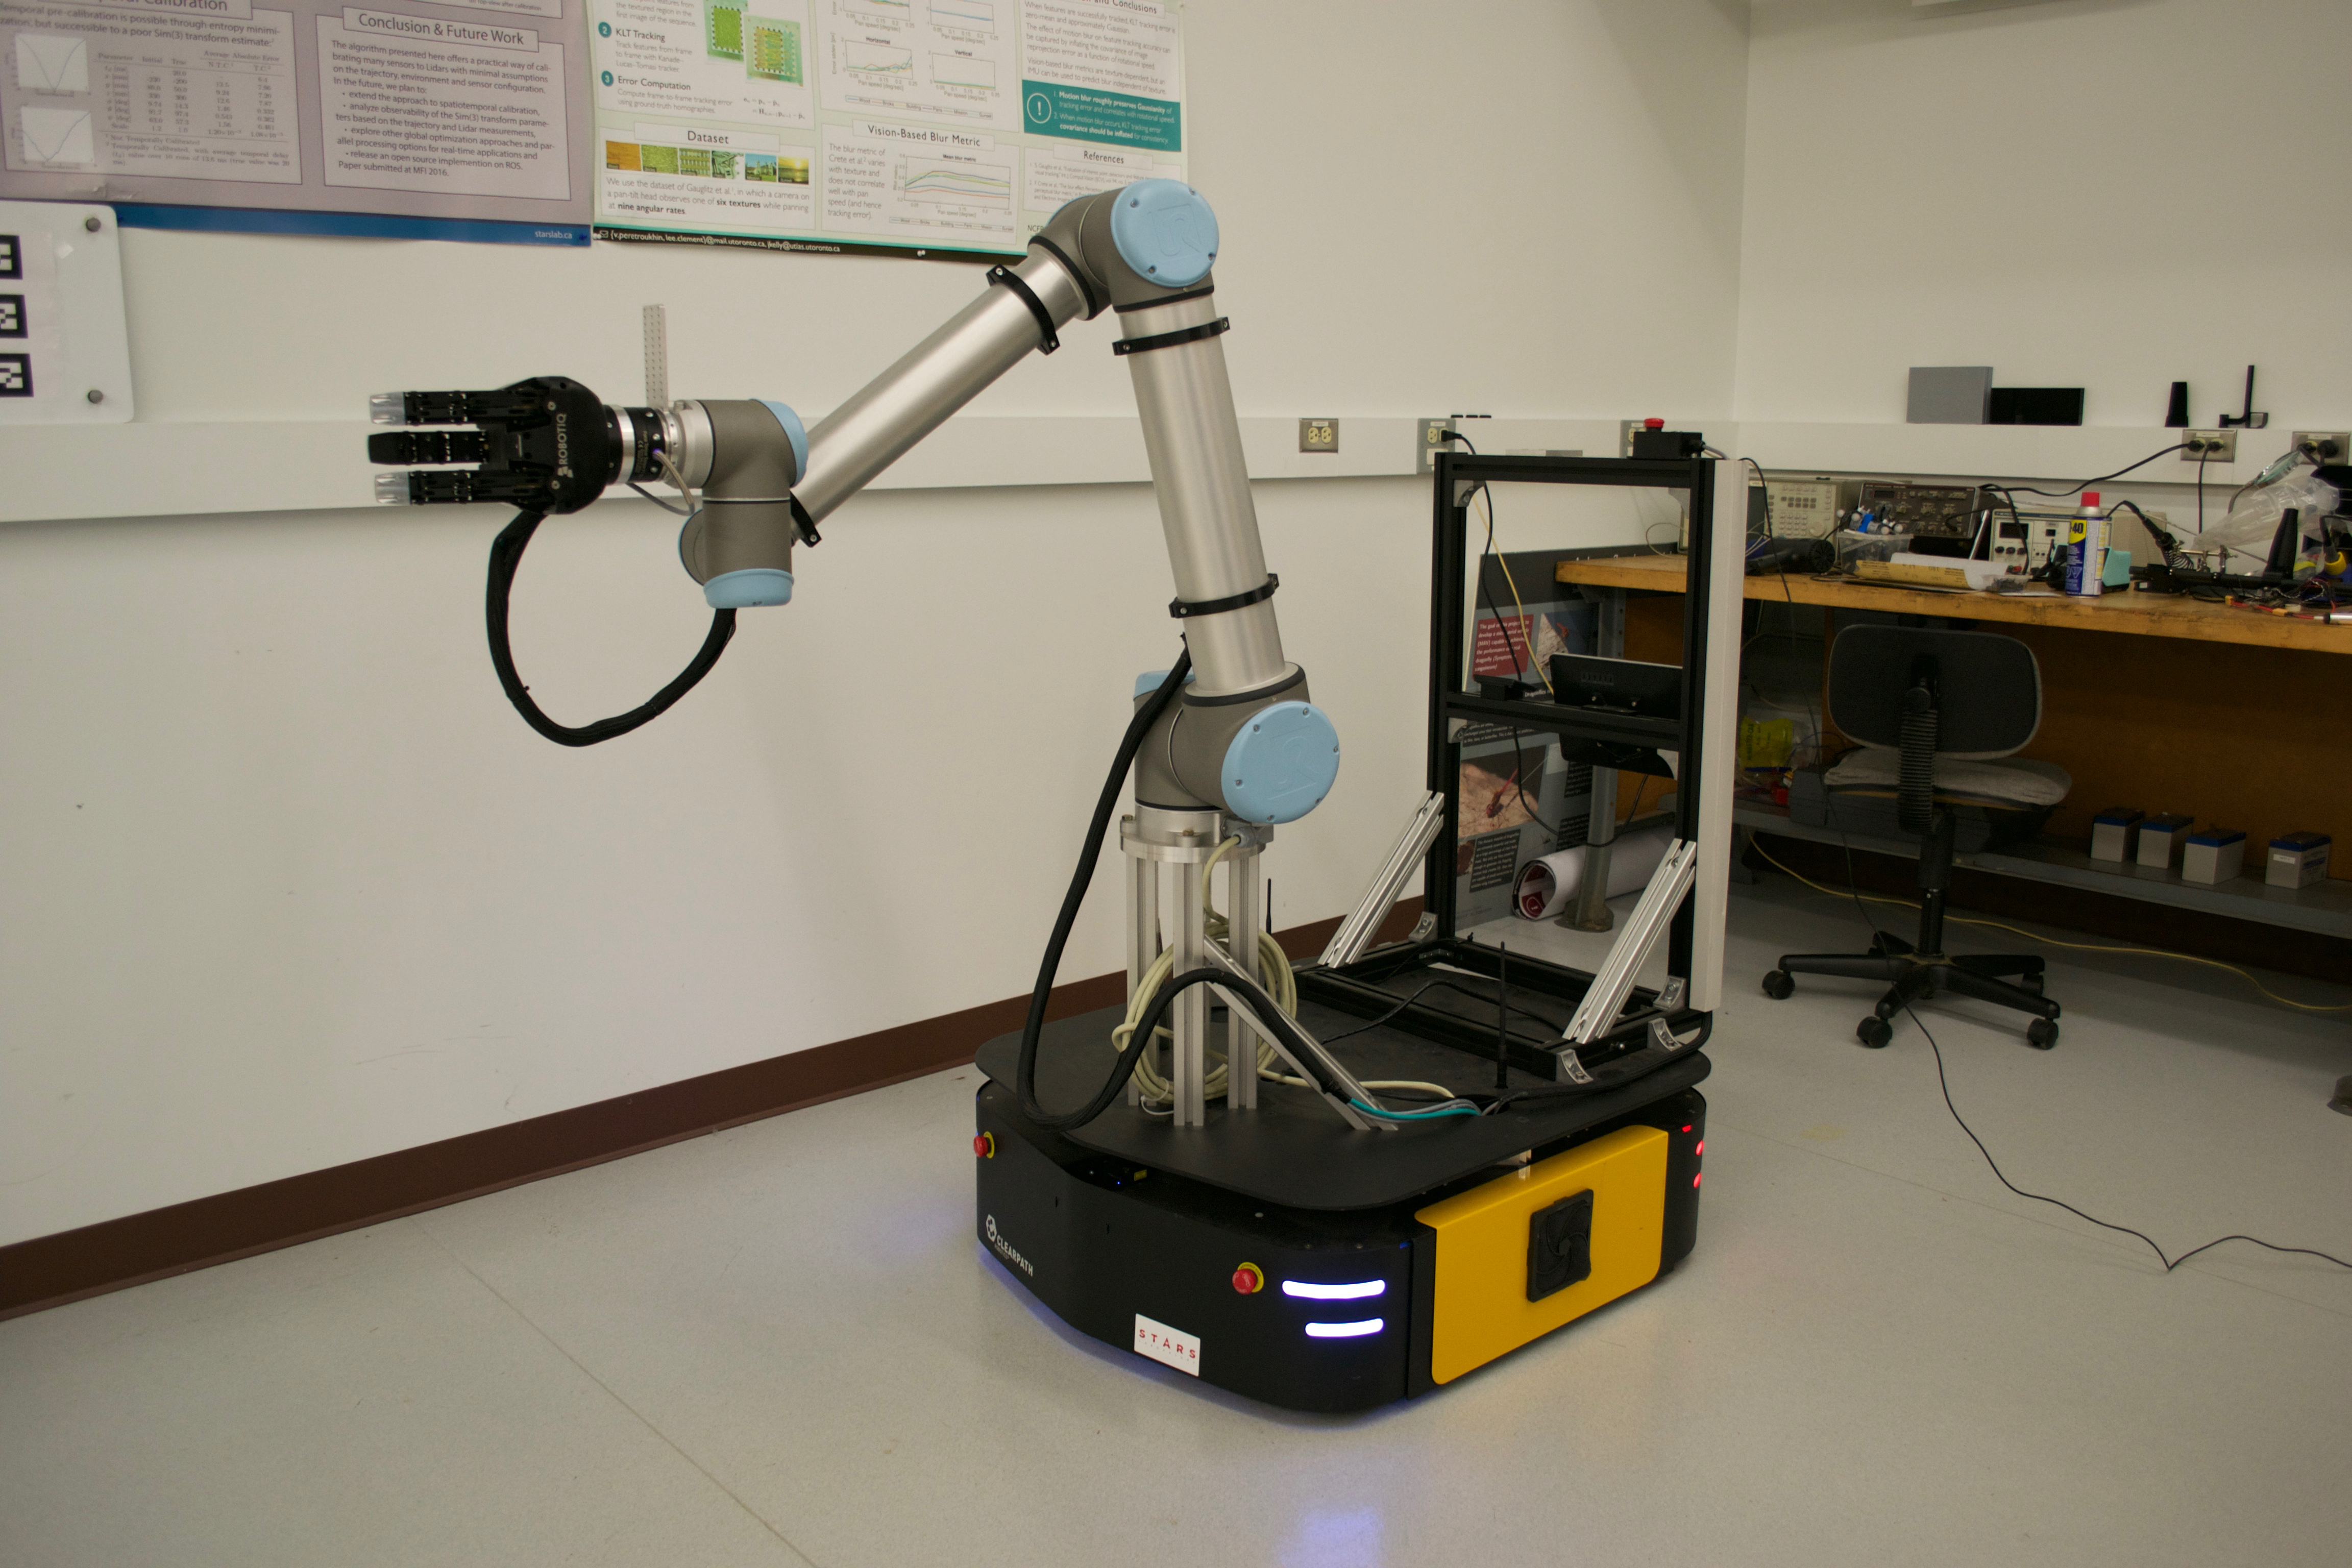
\includegraphics[width=0.75\textwidth]{images/thing.jpg}
   \caption{The Thing mobile manipulator, which consists of a Ridgeback omnidirectional platform, a UR10 and a Robotiq gripper.}
   \label{pics:thing}
\end{figure}

These hardware packages are essentially independent and are interfaced in a central computing unit, located in the ridgeback. The interface is achieved using a Robot Operating System (ROS) server, which also acts as the user interface. It allows for information sharing between the system and access for the user on high and low system levels.

The rich and easily expandable sensing equipments include wheel odometry, an inertial measurement unit (IMU) and a Hokuyo laser range finder (\textsc{Lidar}) \citep{hokuyo} in the Ridgeback and a FT 300 force-torque sensor \citep{robotiqFT300} in between the gripper and the UR10.

The omnidirectional capability together with the modularity of the system and the vast amount of sensor arrays make mobile manipulators like the Thing a popular and widely used system for autonomous robotics research.

The whole manipulator is an out of the box system assembled by Clearpath, which collaborates with Universal Robots and Robotiq and mounts the parts onto the platform in house.

\section{Clearpath Ridgeback}
	\label{sec:ridgeback}
The Ridgeback, depicted in Figure \ref{pics:ridgeback} is an omnidirectional robot platform designed by Clearpath for indoor movement and payload carrying tasks, such as autonomous warehousing for example. It is a fully integrated system with sensors, actuation and control and features a native ROS interface. The wheel odometry provides accurate localization and can be fused with the front facing \textsc{Lidar} and IMU for obstacle avoidance and SLAM implementations, which are available for example in the ROS navigation stack. Optionally, a second rear facing \textsc{Lidar} can be mounted for full \unit[360]{\textdegree} coverage. Specifications are summarized in Table \ref{tab:ridgeback}.

\begin{figure}[h]
   \centering
   \includegraphics[width=0.75\textwidth]{images/ridgeback.png}
   \caption{Clearpath Ridgeback}
   \label{pics:ridgeback}
\end{figure}

\begin{table}[h]
\begin{center}
 \caption{Clearpath Ridgeback specifications}\vspace{1ex}
 \label{tab:ridgeback}
 \begin{tabular}{ll}
 \hline
 Length & \unit[960]{mm}\\
 Width & \unit[793]{mm}\\
 Height & \unit[296]{mm}\\
 Weight & \unit[135]{kg}\\
 Maximum payload & \unit[100]{kg}\\
 Maximum velocity & \unitfrac[1.1]{m}{s}\\
 Average power consumption & \unit[800]{W}\\
 Drivers and APIs & ROS \\
 Sensors & Wheel odometry\\
 & Inertial measurement unit (IMU) \\
 & Laser range finder \textsc{Lidar} \\
 \hline
 \end{tabular}
\end{center}
\end{table}

The broad range of sensors, it's flexibility and low drift in odometry makes the Ridgeback a suitable and popular platform for research in controlled indoor environments.

Because the Ridgeback is omnidirectional, it has three degrees of freedom (DOF) and can move instantaneously along the two linear horizontal axes $x$ and $y$, as well as rotate around the vertical axis $z$, which is expressed by the yaw angle $\theta$. 

Additionally, the Ridgeback houses the on-board computer that runs the low-level drivers of all the elements of the manipulator. On top thereof, there is a high-level driver that ensures accord and offers a ROS interface for the user to connect to.

\section{Universal Robot 10}
The UR10 is a collaborative industrial robot arm by Universal Robots. It has six rotary joints, hence six DOF and can support payloads up to \unit[10]{kg}. Together with it's little brother the UR5, it is widely regarded as the standard manipulator within robotics research. Hence, extensive platform and software integration resources are available and ROS is supported out of the box.

As we see in Table \ref{tab:ur10}, the repeatability of \unit[0.1]{mm} allows for repeatedly achieving a pose with high accuracy, which is important for industrial and research applications alike.

\begin{figure}[h]
   \centering
   \includegraphics[width=0.75\textwidth]{images/ur10.png}
   \caption{Universal Robot 10}
   \label{pics:ur10}
\end{figure}

\begin{table}[h]
\begin{center}
 \caption{Universal Robot 10 specifications}\vspace{1ex}
 \label{tab:ur10}
 \begin{tabular}{ll}
 \hline
 Reach & \unit[1300]{mm} \\
 Weight & \unit[1.5]{kg}\\
 Repeatability & \unit[0.1]{mm} \\
 Maximum payload & \unit[10]{kg}\\
 Maximum tool velocity & \unitfrac[1]{m}{s}\\
 Degrees of freedom & 6 rotating joints \\
 Average power consumption & \unit[350]{W}\\
 \hline
 \end{tabular}
\end{center}
\end{table}

\section{Robotiq Three Finger Gripper}
The Robotiq three finger adaptive gripper, depicted in Figure \ref{pics:robotiq_gripper}, acts as the end-effector mounted on the UR10 on the Thing. As specified in Table \ref{tab:robotiq_gripper}, it has four different grip types and allows for force, position and speed control for each finger individually. This makes it suitable for manufacturing, assembly, pick and place and other research applications.

\begin{figure}[h]
   \centering
   \includegraphics[width=0.75\textwidth]{images/robotiq_gripper.jpg}
   \caption{Robotiq three finger adaptive robot gripper}
   \label{pics:robotiq_gripper}
\end{figure}

\begin{table}[h]
\begin{center}
 \caption{Robotiq three finger adaptive robot gripper specifications}\vspace{1ex}
 \label{tab:robotiq_gripper}
 \begin{tabular}{ll}
 \hline
 Weight & \unit[2.3]{kg}\\
 Repeatability & \unit[0.1]{mm} \\
 Maximum payload (encompassing grip) & \unit[10]{kg}\\
 Gripper opening & \unit[0 to 155]{mm} \\
 Object diameter for encompassing & \unit[20 to 155]{mm}\\
 Grip force & \unit[30 to 70]{N} \\
 Grip types & Pinch mode \\
 & Wide mode \\
 & Scissor mode \\
 & Basic mode \\
 Minimum power consumption & \unit[4.1]{W} \\
 Peak power (at maximum gripping force) & \unit[36]{W}\\
 \hline
 \end{tabular}
\end{center}
\end{table}

\section{Robotiq FT 300 Force-Torque Sensor}
	\label{sec:ft300}
The FT 300 is a force-torque sensor by Robotiq, embedded in a cylindrical and stiff casing. As Figure \ref{pics:robotiq_ft} shows, the sensor is compatible with any Robotiq gripper and Universal Robots arm and acts as an intermediate module between the gripper and the end-effector of the robotic arm. Hence, any force or torque which is transferred from gripper to the arm or vice versa can be measured. The sensor measures forces along and torques around the three axis $x$, $y$ and $z$ of the module, making it a six dimensional sensor, outputting data at \unit[100]{Hz}. In Table \ref{tab:robotiq_ft}, the measuring ranges and signal noises are listed.

The FT-300 allows for any tasks that make use of force feedback or force control, such as assembly, finishing, insertion, pick and place or teach and repeat applications.


\begin{figure}
   \centering
   \includegraphics[width=0.75\textwidth]{images/robotiq_ft.jpg}
   \caption{Robotiq FT 300 force-torque sensor}
   \label{pics:robotiq_ft}
\end{figure}

\begin{savenotes}
\begin{table}[h]
\begin{center}
 \caption{Robotiq FT 300 force-torque sensor specifications}\vspace{1ex}
 \label{tab:robotiq_ft}
 \begin{tabular}{ll}
 \hline
 \textbf{Measuring range} & \\
 Force $F_x, F_y, F_z$ & \unit[$\pm 300$]{N} \\
 Torque $T_x, T_y, T_z$ & \unit[$\pm 30$]{Nm} \\ \hline
 \textbf{Signal noise}\footnote{Signal noise is the standard deviation of the signal measured over a period of one second.} &\\
 Force $F_x, F_y, F_z$ & \unit[0.1]{N} / \unit[1]{N} \\
 Torque $T_x, T_y$ & \unit[0.05]{Nm} / \unit[0.02]{Nm} \\
 Torque $T_z$ & \unit[0.03]{Nm} / \unit[0.01]{Nm} \\ \hline
 Data output rate & \unit[100]{Hz} \\
 Weight & \unit[300]{g}\\
 Outside diameter & \unit[75]{mm} \\
 Thickness & \unit[37.5]{mm} \\
 \hline
 \end{tabular}
\end{center}
\end{table}
\end{savenotes}

\section{Hokuyo Laser Range Finder}
	\label{sec:hokuyo}
Figure \ref{pics:hokuyo} depicts the Hokuyo UST-10LX scanning laser range finder. It scans a single horizontal plane by spinning around its vertical axis at \unit[2400]{rpm}, which results in a scanning frequency of \unit[40]{Hz}, also shown in Table \ref{tab:hokuyo}. Compared to any \textsc{Lidar} system that stacks multiple lasers on top of each other, the Hokuyo UST-10LX is in a disadvantage, because it only outputs two-dimensional range measurements and supplies no information along its vertical axis. However, it outperforms many alternatives in terms of size, weight, power consumption, accuracy and measurement frequency, which makes it highly suitable for a mobile platform.


\begin{figure}[h]
   \centering
   \includegraphics[width=0.75\textwidth]{images/hokuyo.jpg}
   \caption{Hokuyo UST-10LX laser range finder}
   \label{pics:hokuyo}
\end{figure}

\begin{table}[h]
\begin{center}
 \caption{Hokuyo UST-10LX laser range finder specifications}\vspace{1ex}
 \label{tab:hokuyo}
 \begin{tabular}{ll}
 \hline
 Scan angle & \unit[250]{$\degree$} \\
 Measurement steps & 1081 \\
 Angular resolution & \unit[0.25]{$\degree$} \\
 Detection range & \unit[0.06 to 10]{m} \\
 Scan frequency & \unit[40]{Hz} \\
 Average power consumption & \unit[3]{W} \\
 Weight & \unit[130]{g} \\
 Length & \unit[50]{mm} \\
 Width & \unit[50]{mm} \\
 Height &  \unit[70]{mm} \\
 \hline
 \end{tabular}
\end{center}
\end{table}

\chapter{Admittance Control}
	\label{sec:adm_ctrl}
	
The term \emph{admittance control} is closely coupled to the term \emph{impedance control} and essentially they refer to two opposing ways of implementing the same control goal. The goal is to model the dynamic coupling between the end-effector and its environment, which is essential in robotics for environment interaction and object manipulation \citep{hogan1985impedance}.

The coupling is achieved by establishing a dynamic relationship between the position and force of the end-effector. Which we model as a second order spring mass damper system, as depicted in Figure \ref{pics:mass_spring_damper}. For reasons of simplicity, only the one-dimensional case is drawn, however the following derivation scales up to $n$ dimensions and has a physical representation for up to six dimensions.

According to Newton's second law of motion, the change in momentum is equal to the sum of all forces $F \in \mathbb{R}^{n \times 1}$ acting on our rigid body

\begin{equation}
M \cdot \ddot{X} = \sum F
	\label{eq:virt_work}
\end{equation}
where $M \in \mathbb{R}^{n \times n}$ is the inertia matrix and $\ddot{X} \in \mathbb{R}^{n \times 1}$ the acceleration of the rigid body.

The forces in the case of the mass spring damper system become apparent if we free-cut our system, as  seen in Figure \ref{pics:mass_spring_damper_freecut}.
\begin{equation}
\sum F = F_{ext} -F_D - F_K
	\label{eq:f_sum}
\end{equation}
Which consists of a spring term $F_K$ with spring constant $K$,
\begin{equation}
F_K = K \cdot X
\end{equation}
 a damping term $F_D$ with damping constant $D$
\begin{equation}
F_D = D \cdot \dot{X}
\end{equation}
 and a term $F_{ext}$ for external forces acting on the body. Replacing $\sum F$ in Equation \ref{eq:virt_work} with Equation \ref{eq:f_sum} yields the equation for a second order mass spring damper system:
\begin{equation}
M \cdot \ddot{X} = F_{ext} -D \cdot \dot{X} -K \cdot X
	\label{eq:mass_spring_damper_sys}
\end{equation}

\begin{figure}
   \centering
   \includegraphics[width=0.75\textwidth]{images/mass_spring_damper.pdf}
   \caption{Second order mass spring damper system, where a rigid body with mass $M$ is attached through a spring $K$ and a damper $D$.}
   \label{pics:mass_spring_damper}
\end{figure}

\begin{figure}
   \centering
   \includegraphics[width=0.75\textwidth]{images/mass_spring_damper_freecut.pdf}
   \caption{Free-cut second order mass spring damper system. Forces between the rigid body and the spring and the damper are introduced as $F_K$ and $F_D$ respectively.}
   \label{pics:mass_spring_damper_freecut}
\end{figure}
%
%We can transform Equation \ref{eq:mass_spring_damper_sys} into state-space representation using 
%
%\begin{equation}
%Z = \dot{X}
%\end{equation}
%
%and we get:
%
%\begin{equation}
%M \cdot \dot{Z} = F_{ext} -  D \cdot Z - K \cdot X
%\label{eq:mass_spring_damper_state_space}
%\end{equation}
%
%Written in matrix form, Equation \ref{eq:mass_spring_damper_state_space} becomes
%
%\begin{equation}
%\begin{bmatrix}
%\dot{X} \\
%\dot{Z} \\
%\end{bmatrix} = \begin{bmatrix}
%0 & 1 \\
%- \frac{K}{M} & - \frac{D}{M}\\
%\end{bmatrix} \begin{bmatrix}
%X \\
%Z \\
%\end{bmatrix} + \begin{bmatrix}
%0 \\
%\frac{F_{ext}}{M} 
%\end{bmatrix}
%\end{equation}

Through the usage of energy storing elements, such as the mass and the spring, and energy dissipating elements, such as the damper, the model allows for control of the energy exchange during interaction and we can translate force into position and vice versa. 

Accordingly, the definition of impedance is the ratio of force output to motion input, i.e. a physical system, that accepts \emph{motion inputs} and yields \emph{force outputs} \citep{ott2010unified}.

Admittance is then the inverse of impedance, so the ratio of motion output to force input or a physical a system that accepts \emph{force inputs} and yields \emph{motion outputs}.

\begin{description}
\item[Impedance Control] When looking at the coupling, the impedance controller treats the environment as an admittance and the manipulator as an impedance. The schematic is depicted in Figure \ref{pics:impedance_control}, where we see that the controller relates the deviation $X_{err} = X - X_0$ from an equilibrium trajectory $X_0$ to the external force $F_{ext}$ and outputs the resulting force $F$ to the plant. This leads to a stable dynamic interaction with stiff environments but often to instability in free space.

\item[Admittance Control] On the contrary, the admittance controller treats the environment as an impedance and the manipulator as an admittance, as shown in Figure \ref{pics:admittance_control}. We notice that the controller takes the equilibrium trajectory $X_0$ and the external force $F_{ext}$ as inputs and outputs the desired trajectory $X_{des}$, which satisfies the mass spring damper system of the position controlled plant.
\end{description}

To summarize, we see that impedance control and admittance control are inverse variations of controlling a dynamic coupling between a manipulator and its environment, using the mass spring damper model. The impedance controller relates a given motion input to a force output to the environment and the admittance controller positions the manipulator given a force input from the environment. Since our system is to follow a trajectory $X_{des}$ given the force input $F_{ext}$ from the human partner, we are applying the latter and we elaborate on our implementation in Chapter \ref{sec:implementation}.

\begin{figure}
   \centering
   \includegraphics[width=0.75\textwidth]{images/impedance_control_schematic.pdf}
   \caption{Impedance control schematic. Inputs to the controller are the deviation $X_err$ calculated from the equilibrium trajectory $X_0$ and the actual trajectory $X$, and the external force $F_{ext}$. Output is the force $F$ which the manipulator exerts on its environment.}
   \label{pics:impedance_control}
\end{figure}

\begin{figure}
   \centering
   \includegraphics[width=0.75\textwidth]{images/admittance_control_schematic.pdf}
   \caption{Admittance control schematic. The controller outputs a desired trajectory $X_des$ to the position controlled plant, given the equilibrium trajectory $X_0$ and the external force $F$.}
   \label{pics:admittance_control}
\end{figure}


\chapter{Obstacle Avoidance}
Ever since robots faced the task of autonomous navigation, obstacle avoidance has been a crucial element of it. There are numerous approaches to tackle the problem, varying in degrees of foresight and influence on the path planner.

The problem can be separated into two categories, path planning around obstacles on a global scale and on a local scale. The first category bundles algorithms that take a goal position and a current position of a robot and calculate the optimal path (usually the shortest path) in between, given some objective function and a map. Since the distance to the goal is normally greater than the range of any obstacle detection sensor, these algorithms need a full map of the environment. Widely used examples are A*, Dijkstra and RRT.

In contrast, path planning on a local scale takes obstacle detection sensor information as an input and outputs commands to a drive unit, that meet the given objective, which is usually to avoid collisions and stay clear of an obstacle by a minimum distance. 

A typical path planning infrastructure on a robot consists of both a global and a local planner, where the global planner outputs a path to follow to the local planner, which in terms fuses that path with online obstacle detection sensor information to ensure it is indeed collision free and deviates from it if necessary.

To find the path planning algorithm that best meets our needs, we must first examine what are the given inputs and the desired outputs of our system. As we already elaborated in \cref{sec:introduction}, we are working in a master-slave scenario, which means that the robot is trying to achieve the goal of its human counterpart and not its own. This manifests in the planner in such a way, that the input is the force and torque applied by the human and the robot has no global goal pose. Hence, we are inherently bound to iteratively updated goals within close proximity and there is no possibility nor need to apply global path planning techniques and we focus only on local planners in the remainder of this chapter.

\section{Local Planners}
We discuss a selection of common local planning methods and their feasibility for the task at hand.

\subsection{Dynamic Window Approach}
The Dynamic Window Approach (DWA) \citep{fox1997dynamic} is a well-known algorithm that produces command velocities for a planar robot given vehicle dynamics and obstacle measurements. The basic assumption is that the robot moves instantaneously on circular arcs with a translational velocity $v$ and a rotational velocity $\omega$. Thus, the complexity is greatly simplified and calculations are be performed in the 2D velocity space $(v,\omega)$. Within this space, we compute three sets of velocity pairs,  subsequently called \emph{windows} for every iteration of the algorithm. Figure \ref{pics:dwa} provides a visual example of the functionality of the algorithm.

\begin{description}
\item[Static window] The static window $V_s$ expresses the constraint velocities of the vehicle, i.e., absolute maximum and minimum velocity. As the name suggests, these parameters are usually static and do not need to be recalculated every step.

\item[Obstacle window] The obstacle window $V_o$ are the measurements of any obstacles, e.g. taken by a range laser sensor and transformed from Cartesian to $v,\omega$ space.

\item[Dynamic window]The dynamic window $V_d$ are the vehicle dynamics, i.e., velocities that are physically feasible for the robot to reach within one time step. It's size is defined by the maximal acceleration and the current velocity of the robot.
\end{description}

\begin{figure}
   \centering
   \includegraphics[width=0.75\textwidth]{images/dwa.png}
   \caption{DWA working principle \citep{siegwart2004autonomous}. \emph{Left:} Example of a planar robot and one obstacle in Cartesian space. \emph{Right:} Representation of the same scenario in $(v,\omega)$ velocity space. The large bounding box depicts the static window $V_s$, the dark grey area depicts the obstacle window $V_o$, the small bounding box depicts the dynamic window $V_d$ and the black dot represents the current velocity pair of the robot. The resulting window $V_r$ is then the intersection of all three areas.}
   \label{pics:dwa}
\end{figure}

\begin{equation}
V_r = V_o \cap V_s \cap V_d
 	\label{eq:dwa_intersection}
\end{equation}

As Equation \ref{eq:dwa_intersection} shows, the intersection of these three sets gives us the resulting window $V_r$ of feasible velocity pairs, that guarantee no collision with an obstacle for the next step.

A cost function is then applied to find the $(v,\omega)$ pair, that maximizes the objective within $V_r$. Elements of the cost function are heading, distance to goal and velocity terms.

A general downside of the DWA is that the method assumes objects to be static, which can lead to problems in a dynamically changing environment. If we think about an implementation of DWA within the task hand, it means that we need to create a goal velocity pair $(v_{goal},\omega_{goal})$ for the DWA from our external force input $F_{ext}$. Hence, a transformation from force to velocity is needed, which could be achieved through integration. However, there is still the need for tuning, because it is not clear what magnitude of the goal velocity pair $|(v_{goal},\omega_{goal})|$ works best with DWA. Furthermore, The admittance control and the DWA would be organized sequentially in the control architecture, which means that the admittance control solely outputs a goal velocity pair $(v_{goal},\omega_{goal})$ to the DWA and has no knowledge of the actual command velocity being sent to the hardware.

For these reasons, DWA does not meet our requirements for an obstacle avoidance algorithm and we decide against an implementation of DWA.


\subsection{Potential Fields}
	\label{sec:pot_field}
Potential fields are also a common tool in the mobile robotics field used for path planning. The concept is a virtual potential $U(p)$ at position $p = (x,y)$ affecting the robot and driving him away from any maximum, like a ball rolling downhill \citep{siegwart2004autonomous}.

It can be used to attract the robot to a goal by creating a local minimum and repulsing a robot from an obstacle by creating a local maximum. An example of multiple attractive and repulsive potentials is given in Figure \ref{pics:pot_field}.

The superposition of all attractive and repulsive potential fields yields the overall potential $U(p)$:
\begin{equation}
U(p) = U_{attr}(p) + U_{rep}(p)
	\label{eq:pot_field}
\end{equation}

If the potential field is differentiable, we find that the resulting virtual force $F(p)$ that acts on the robot in position $p$ is then defined as 
\begin{equation}
F(p) = - \nabla U(p) 
	\label{eq:pot_force}
\end{equation}
where $\nabla U(p)$ is the gradient of the potential field
\begin{equation}
\nabla U(p) = \begin{pmatrix}
\frac{\partial U}{\partial x} \\
\frac{\partial U}{\partial y}
\end{pmatrix}
	\label{eq:gradient}
\end{equation}

Similarly, by combining Equation \ref{eq:pot_force} and Equation \ref{eq:pot_field} we see that the overall force equals the sum of the attractive and repulsive forces:
\begin{equation}
\begin{aligned}
F(p) &= F_{att}(p) + F_{rep}(p) \\
&= -\nabla U_{att}(p)-\nabla U_{rep}(p)
\end{aligned}
\end{equation}


An \textbf{attractive potential}, i.e. a goal is usually defined as a parabolic function

\begin{equation}
U_{att}(p) = \frac{1}{2} k_{att} \cdot {\rho_{goal}}^2(p)
\end{equation}

where $k_{att}$ is the scaling factor and $\rho_{goal}$ is the Euclidian distance to the goal:
\begin{equation}
\rho_{goal} = ||p-p_{goal}||
\end{equation}


A \textbf{repulsive potential}, i.e. an obstacle is zero if a certain distance is exceeded and should rise drastically when the robot gets within close proximity of the obstacle. Hence, a common definition is
\begin{equation}
U_{rep}(p) = \begin{cases}
      \frac{1}{2} k_{rep}\cdot (\frac{1}{\rho (p)}-\frac{1}{\rho_0})^2 & \text{if}\ \rho (p) \leq \rho_0 \\
      0 & \text{if}\ \rho (p) \geq \rho_0 \\
    \end{cases}
    \label{eq:pot_field_repulsive}
\end{equation}
where $k_{rep}$ is the scaling factor, $\rho_0$ is the distance threshold and $\rho (p)$ is the minimal distance from position $p$ to the obstacle.

\begin{figure}[h]
   \centering
   \includegraphics[width=0.75\textwidth]{images/pot_field.png}
   \caption{Potential field method working principle \citep{siegwart2004autonomous}. Grey areas represent obstacles, the blue circle represents a goal. Depicted in grey and black lines are the equipotential lines of the repulsive and attractive potentials respectively. The robot will follow the direction of the largest gradient, based on his starting position.} 
   \label{pics:pot_field}
\end{figure}

The main limitation to this approach is that it is prone to local minima, where the robot can get stuck. However, we are not working with any global goals, but rather with an user input in form of a force so even if the robot is within a local minima, the user can literally pull it away from it. Furthermore, because the output of the potential field method is a force vector, we can elegantly combine it with the admittance controller, which also operates using virtual forces acting on the robot. 

So, we conclude that the potential field method is most suitable for a fusion with an admittance controller and we will elaborate on our implementation in the following.

\chapter{Implementation}
\label{sec:implementation}
\begin{figure}
   \centering
   \includegraphics[width=0.75\textwidth]{images/controller_overview.pdf}
   \caption{Schematic of the controller. Boxes filled in grey are the nodes of the controller and the arrows indicate information flow between the nodes of the control architecture. The top level nodes are the sensor inputs, which are the readings from the \emph{force-torque sensor} and the \emph{\textsc{Lidar}}. Beneath, we have the nodes which make up the controller, namely the \emph{admittance control}, the \emph{obstacle avoidance} and the \emph{inverse kinematics}. Nodes on the bottom represent the harwarde interfaces for the \emph{mobile base} and the \emph{manipulator}.}
   \label{pics:controller_overview}
\end{figure}

Having selected the potential field method as the desired obstacle avoidance algorithm, we can move on to fusing it together with the admittance controller. Figure \ref{pics:controller_overview} shows the overall controller schematic as a flowchart, with the nodes used and their messages exchanged, and Table \ref{tab:controller_nodes} summarizes the individual nodes and their ROS messages used.

Firstly, we outline the overall functionality of the system by explaining the functionality of all nodes briefly and dive more deeply into nodes of interest subsequently.

\begin{description}
  \item[Force-torque sensor] The force-torque sensor node continuously outputs the readings from the FT 300 (Chapter \ref{sec:ft300}) as a wrench $F_{ext}$ of dimension $\mathbb{R}^{6 \times 1}$. The top three elements are the linear force readings in $[N]$ and the latter the angular torque readings in $[Nm]$. All packed in a ROS message of type \emph{WrenchStamped} \citep{rosWrench} and published at a rate of \unit[100]{Hz}. 

  \item[LIDAR] The output of the \textsc{Lidar} node are the scans from the Hokuyo laser range finder (Chapter \ref{sec:hokuyo}). Each \emph{Laser-scan} ROS message \citep{rosLaserscan} contains the range and intensity of every laser measurement taken from the minimum to the maximum angle of the sensor.
  
  \item[Obstacle avoidance] Given the laser-scan readings, the obstacle avoidance node creates a costmap \citep{rosCostmap} around the mobile manipulator, which is explained in detail in Chapter \ref{sec:costmap}. The costmap is the obstacle potential of all obstacles seen in the laser-scans and we derive the resulting force $F_{obs}$ analogously to Equation \ref{eq:pot_force} as
  \begin{equation}
  F_{obs} = - \nabla U_{obs}(p)
  \end{equation}
  where $p$ is the current position of the centre of the Ridgeback. Because the costmap is in two dimensional horizontal space, the resulting force $F_{obs}$ is also planar and has dimension $\mathbb{R}^{2 \times 1}$. 
  
  \item[Admittance control] We feed these into the \emph{admittance control}, whose other inputs are the vehicle kinematics, namely the current pose $X_{base}$ \citep{rosPose} and twist $\dot{X}_{base}$ \citep{rosTwist} of the ridgeback \emph{mobile base} and the current pose $X_{ee}$ and twist $\dot{X}_{ee}$ of the UR10 \emph{manipulator}. Given these inputs, we calculate the desired twist $\dot{X}_{base_{des}}$ for the mobile base and the desired twist $\dot{X}_{ee_{des}}$ for the manipulator in Cartesian space.
  
  \item[Inverse kinematics] To obtain a feasible velocity $\dot{q}_{ee_{des}}$ in joint space for the manipulator, the desired twist $\dot{X}_{ee_{des}}$ needs to transformed from Cartesian to joint space. To ensure alignment with the desired twist $\dot{X}_{base_{des}}$ of the base, \emph{inverse kinematics} is performed collectively, as detailed in Chapter \ref{sec:inversekinematics}.
  
  \item[Mobile base] This node represents the hardware interface and the low level controller of the Ridgeback. It accepts a command velocity as input and using the wheel odometry, it can accurately estimate its pose $X_{base}$ and velocity $\dot{X}_{base}$ and publish these.
  \item[Manipulator] This node represents the hardware interface and the low level controller of the UR10. Joint command inputs can be given through a \emph{FollowJointTrajectory} action server \citep{rosJointTrajectory}, to which we continuously publish the command joint positions $q_{ee_{des}}$. Similarly to the mobile base node, outputs are the pose $X_{ee}$ and velocity $\dot{X}_{ee}$.
\end{description}

\begin{table}
\begin{center}
 \caption{Controller nodes and their respective outputs.}\vspace{1ex}
 \label{tab:controller_nodes}
 \begin{tabular}{l|lccl}
 \hline
Node & Output & Dimension & Unit & ROS message type \\ \hline \hline
Force-torque sensor & $F_{ext}$ & $\mathbb{R}^{6 \times 1}$ & $[N]$ & WrenchStamped \\
\textsc{Lidar} & $F_{obs}$ & $\mathbb{R}^{2 \times 1}$ & $[N]$ & WrenchStamped \\
Admittance control & $\dot{X}_{base},\dot{X}_{ee}$ & $\mathbb{R}^{10 \times 1}$ & $[N]$ & Custom twist message \\
Inverse kinematics & $\dot{X}_{base_{des}}$ & $\mathbb{R}^{3 \times 1}$  & $[\sfrac{m}{s}]$ & TwistStamped \\
& $\dot{q}_{ee_{des}}$&$\mathbb{R}^{6 \times 1}$ & $[rad]$ & FollowJointTrajectory\\
Mobile base & $X_{base}$ & $\mathbb{R}^{7 \times 1}$ & $[m]$ & PoseStamped \\
& $\dot{X}_{base}$ & $\mathbb{R}^{6 \times 1}$ & $[\sfrac{m}{s}]$ & TwistStamped \\
Manipulator & $X_{ee}$ & $\mathbb{R}^{7 \times 1}$ & $[m]$ & PoseStamped \\
& $\dot{X}_{ee}$ & $\mathbb{R}^{6 \times 1}$ & $[\sfrac{m}{s}]$ & TwistStamped \\


 \hline
 \end{tabular}
\end{center}
\end{table}

\section{Admittance Control and Obstacle Avoidance Fusion}
\label{sec:fusion}
\begin{figure}
   \centering
   \includegraphics[width=0.75\textwidth]{images/admittance_model.jpg}
   \caption{Virtual spring mass damper system with two inertia matrices. Dotted arrows represent the path of the base (left) and the arm (right) over time, connected by the spring mass damper system.}
   \label{pics:admittance_model}
\end{figure}
The key element of the whole algorithm is the fusion of the admittance controller, as described in Chapter \ref{sec:adm_ctrl} and the obstacle avoidance, as described in Chapter \ref{sec:pot_field}. In order to achieve this, we define a virtual two mass spring damper system, depicted in Figure \ref{pics:admittance_model}. Here $M_{ee}$ represents the virtual inertia matrix of the EE with pose $X_{ee}$ and $M_{base}$ the virtual inertia matrix of the Ridgeback with pose $X_{base}$. We couple the two inertia matrices together using a spring element with a spring constant $K$ and a damping element with a damping constant $D$. This coupling has an equilibrium position which is defined a priori and is denoted by $X_{eq}$. As the name suggests,  the coupling is in an equilibrium when

\begin{equation}
\overline{\rm X_{base}X_{ee}} = X_{eq}
\end{equation}

Furthermore, we add additional damping elements $D_{ee}$ and $D_{base}$, through which we couple the two inertia matrices to their desired trajectories, depicted as dotted arrows in Figure \ref{pics:admittance_model}.

Since the EE is where the system is connected to the human partner, any external force $F_{ext}$ exerted by him attacks at $M_{ee}$. Similarly, because the Ridgeback is running the obstacle avoidance, any force $F_{obs}$ created by it has to attack at $M_{base}$ in the system. 

Applying Equation \ref{eq:mass_spring_damper_sys} to both rigid elements in our virtual system yields the control equations of the fused admittance control and obstacle avoidance algorithm

\begin{equation}
M_{base} \cdot \ddot{X}_{base} = -D_{base} \cdot \dot{X}_{base} - D \cdot \dot{X}_{ee} + K \cdot X_{error}+F_{obs}
	\label{eq:adm_base}
\end{equation}

\begin{equation}
M_{ee} \cdot \ddot{X}_{ee} = -(D + D_{ee}) \cdot \dot{X}_{ee} - K \cdot X_{error}+F_{ext}
	\label{eq:adm_ee}
\end{equation}

where $X_{error}$ is the deviation from the equilibrium pose $X_{eq}$

\begin{equation}
X_{error} = \overline{\rm X_{base}X_{ee}} - X_{eq}
\end{equation}

Equation \ref{eq:adm_base} is the force equilibrium for the Ridgeback and Equation \ref{eq:adm_ee} the force equilibrium for the EE. We can see that through this coupling, any force $F_{ext}$ exerted by the human parter on the EE will also result in a velocity response of the Ridgeback and vice versa any obstacle force $F_{obs}$ will also result in a velocity response of the EE.

\subsection{Control Parameters}
	\label{sec:params}
In this chapter, we list and elaborate on the tuned parameters used in Equation \ref{eq:adm_base} and \ref{eq:adm_ee}. Since we are in six dimensional space and we are not interested in having any interdependence between the individual axes, all constants are six dimensional diagonal matrices. Thereby, we guarantee a full decoupling of all axes.

We set the equilibrium pose $X_{eq}$ of the EE in respect to the frame of the armbase to be offset by \unit[1]{m} in $x$ and \unit[0.5]{m} in $z$. Equation \ref{eq:eq_pose} shows the full pose in $\mathbb{R}^{7 \times 1}$, consisting of a position and a quaternion\footnote{The UR10 base frame is rotated by \unit[180]{$\degree$} around the vertical axis $z$ in respect to the Ridgeback base frame, hence the negative sign in $x$.}.
\begin{equation}
X_{eq} = \begin{pmatrix}
-1 \\ 0 \\ 0.5 \\ 0 \\ 0 \\ 0.7071067 \\ 0.7071069 \\
\end{pmatrix} \begin{bmatrix}
m \\
- \\
\end{bmatrix}
	\label{eq:eq_pose}
\end{equation}

Since all our parameters are virtual, we can start off by setting the inertia matrix of the EE $M_{ee}$ as the identity matrix. From there, we tune the remaining parameters $M_{base}$, $D_{ee}$,$D_{base}$,$D$ and $K$, which is essentially the same as tuning a PID controller. The goal is to have a fast response on the EE, so that jerky input from the human partner can be compensated and a slower response by the Ridgeback to follow the overall trajectory.

\begin{equation}
M_{ee} = \begin{pmatrix}
1 & 0 & 0 & 0 & 0 & 0 \\
0 & 1 & 0 & 0 & 0 & 0 \\
0 & 0 & 1 & 0 & 0 & 0 \\
0 & 0 & 0 & 1 & 0 & 0 \\
0 & 0 & 0 & 0 & 1 & 0 \\
0 & 0 & 0 & 0 & 0 & 1 \\
\end{pmatrix}
\begin{bmatrix}
kg \\
kg \cdot m^2 \\
\end{bmatrix}
\end{equation}

\begin{equation}
D_{ee} = \begin{pmatrix}
8 & 0 & 0 & 0 & 0 & 0 \\
0 & 8 & 0 & 0 & 0 & 0 \\
0 & 0 & 8 & 0 & 0 & 0 \\
0 & 0 & 0 & 20 & 0 & 0 \\
0 & 0 & 0 & 0 & 20 & 0 \\
0 & 0 & 0 & 0 & 0 & 8 \\
\end{pmatrix}
\begin{bmatrix}
\frac{N s}{m} \\
N m s
\end{bmatrix}
\end{equation}

An important note here is that although Equation \ref{eq:adm_base} is six dimensional, the output sent to the Ridgeback is only three dimensional, as explained in Chapter \ref{sec:ridgeback}. Hence, parameters in linear $z$, angular $x$ and angular $y$, i.e., the third through fifth rows of Equation \ref{eq:M_base} and Equation \ref{eq:D_base} are irrelevant for the performance of the controller. This also means, that the EE behaves as a single mass spring damper system along these axes and we have a two mass spring damper system only along linear $x$, linear $y$ and angular $z$.

\begin{equation}
M_{base} = \begin{pmatrix}
0.1 & 0 & 0 & 0 & 0 & 0 \\
0 & 0.1 & 0 & 0 & 0 & 0 \\
0 & 0 & 10 & 0 & 0 & 0 \\
0 & 0 & 0 & 10 & 0 & 0 \\
0 & 0 & 0 & 0 & 10 & 0 \\
0 & 0 & 0 & 0 & 0 & 0.1 \\
\end{pmatrix}
\begin{bmatrix}
kg \\
kg \cdot m^2 \\
\end{bmatrix}
\label{eq:M_base}
\end{equation}

\begin{equation}
D_{base} = \begin{pmatrix}
20 & 0 & 0 & 0 & 0 & 0 \\
0 & 10 & 0 & 0 & 0 & 0 \\
0 & 0 & 0 & 0 & 0 & 0 \\
0 & 0 & 0 & 0 & 0 & 0 \\
0 & 0 & 0 & 0 & 0 & 0 \\
0 & 0 & 0 & 0 & 0 & 4 \\
\end{pmatrix}
\begin{bmatrix}
\frac{N s}{m} \\
N m s
\end{bmatrix}
\label{eq:D_base}
\end{equation}

\begin{equation}
D = \begin{pmatrix}
0 & 0 & 0 & 0 & 0 & 0 \\
0 & 0 & 0 & 0 & 0 & 0 \\
0 & 0 & 0 & 0 & 0 & 0 \\
0 & 0 & 0 & 0 & 0 & 0 \\
0 & 0 & 0 & 0 & 0 & 0 \\
0 & 0 & 0 & 0 & 0 & 0 \\
\end{pmatrix}
\begin{bmatrix}
\frac{N s}{m} \\
N m s
\end{bmatrix}
\end{equation}

We set the stiffness of the coupling in Equation \ref{eq:K} deliberately to \unitfrac[500]{N}{m} in linear $z$, because we want the jointly carried object to be close to the height of the equilibrium pose, independent of its weight. Similarly, we set the stiffness in angular $x$ and angular $y$ to \unit[500]{Nm}, in order to prevent rotation of the object around these two axes.

\begin{equation}
K = \begin{pmatrix}
150 & 0 & 0 & 0 & 0 & 0 \\
0 & 150 & 0 & 0 & 0 & 0 \\
0 & 0 & 500 & 0 & 0 & 0 \\
0 & 0 & 0 & 500 & 0 & 0 \\
0 & 0 & 0 & 0 & 500 & 0 \\
0 & 0 & 0 & 0 & 0 & 100 \\
\end{pmatrix}
\begin{bmatrix}
\frac{N}{m} \\
N m
\end{bmatrix}
\label{eq:K}
\end{equation}

\subsection{Costmap of the Obstacle Potential}
	\label{sec:costmap}
Using the ROS costmap package \citep{rosCostmap}, this node builds a two dimensional occupancy grid based on the incoming laserscans and inflates the cost according to user specified parameters. Table \ref{tab:costmap_params} lists all parameters and their set values. Since we do only local planning, a local costmap, meaning the center of the costmap is equal to the center of the robot, of size \unit[3 $\times$ 3]{m} suffices.

The algorithm assigns a value from 0 to 100 to every cell of the occupancy grid, which represents the cost $c$ of that cell. We can distinguish four types of cells:

\begin{description}
  \item[Lethal] A lethal cost is assigned to all cells, which are currently occupied by an obstacle and would therefore guarantee a collision, if the robot center would be at one of these cells.
  \begin{equation}
  c_{lethal} = 100
  \end{equation}
  \item[Inscribed] This category applies to all cells, whose distance to an obstacle is less than the radius of the robot, which is defined by the parameter \emph{robot footprint}. Similarly to the lethal cells, a collision is guaranteed if the robot center overlaps with an inscribed cell.
    \begin{equation}
  c_{inscribed} = 99
  \end{equation}
  \item[Obstacle proximity] Obstacle proximity groups all cells, that make up the repulsive potential $U_{rep}$ of the obstacle, as defined in Equation \ref{eq:pot_field_repulsive}. The distance threshold \emph{inflation radius} defines the size of the potential and the \emph{inflater layer cost scaling factor} defines the steepness of the quadratic curve. These cells represent that the robot center is close to an obstacle but not necessarily colliding.
    \begin{equation}
  c_{proximity} = \begin{bmatrix}
  1,98 \\ 
  \end{bmatrix}
  \end{equation}
  \item[Freespace] All cells that are further away from an obstacle than the distance threshold \emph{inflation radius} are set to 0, meaning that the robot can travel freely through theses cells.
    \begin{equation}
  c_{free} = 0
  \end{equation}
\end{description}

\begin{table}
\begin{center}
 \caption{Costmap Parameters.}\vspace{1ex}
 \label{tab:costmap_params}
 \begin{tabular}{ll}
 \hline
Type & Local \\
Update frequency & \unit{60}{Hz} \\
Publish frequency & \unit{60}{Hz} \\ 
Width & \unit{3}{m} \\
Height & \unit{3}{m} \\
Resolution & \unit{0.03}{m} \\
Global frame & Base link \\
Static map & False \\
Rolling window & True \\
Robot footprint & \unit{0.96 $\times$ 0.8}{m} \\
Plugins used & Obstacles layer, inflater layer \\
Inflater layer cost scaling factor & 10  \\
Inflation radius & \unit{2}{m} \\
 \hline
 \end{tabular}
\end{center}
\end{table}

Figure \ref{pics:costmap} depicts an example of the costmap of a scenario, where the Thing is between two obstacles.

\begin{figure}
   \centering
   \includegraphics[width=0.75\textwidth]{images/costmap.png}
   \caption{Costmap visualization during a test, depicted with the simulation of the Thing.  \textsc{Yellow:} Lethal cells ($c = 100$), \textsc{Turquoise:} Inscribed cells ($c = 99$), \textsc{Red to Blue gradient:} Proximity to an obstacle ($c = [1,98]$), \textsc{Transparent:} Free space ($c = 0$).}
   \label{pics:costmap}
\end{figure}

\section{Task Priority Inverse Kinematics}
	\label{sec:inversekinematics}
Forward kinematics, which is the mapping from joint coordinates $q$ to the end-effector configuration $X_{ee}$ of a mobile manipulator, is a well understood problem and can be solved using the \emph{Jacobian} $J(q)$ which is defined as

\begin{equation}
J(q) =
\begin{bmatrix}
\frac{\partial X_1}{\partial q_1} & \hdots & \frac{\partial X_1}{\partial q_{n_j}} \\
\vdots & \ddots & \vdots \\
\frac{\partial X_m}{\partial q_1} & \hdots & \frac{\partial X_m}{\partial q_{n_j}}
\end{bmatrix}
\end{equation}

It relates differences from joint coordinates $q$ to EE configuration  space $X_{ee}$:

\begin{equation}
\dot{X}_{ee} = J(q) \cdot \dot{q}
\end{equation}

The inverse kinematics, i.e., the calculation of the joint velocity $\dot{q}$ given an EE velocity $\dot{X}_{ee}$ is already trickier, but can be achieved using the \emph{Moore-Penrose pseudo inverse} $J^+$ of the Jacobian:

\begin{equation}
\dot{q} = J^+ \cdot \dot{X}_{ee} 
\end{equation}

where $J^+$ is defined as

\begin{equation}
J^+ = J^T(JJ^T)^{-1}
\end{equation}

Furthermore, because we are working with a mobile manipulator and not a rigidly fixed robot arm, there are two Cartesian velocities $\dot{X}_1$ and $\dot{X}_2$, for which we want to solve simultaneously. Hence, we use a multi-task inverse kinematics control that can prioritize among multiple tasks \citep{nakamura1987task}. This is achieved by utilizing \emph{null-space optimization} to execute a secondary task with Jacobian $J_2$, given a primary task with Jacobian $J_1$.

\begin{equation}
\dot{q} = J_1^+ \dot{X}_1 + N_1 J_2^+ N_1 (\dot{X}_2-J_2J_1^+\dot{X}_1)
\label{eq:task_priority}
\end{equation}

Equation \ref{eq:task_priority} formulates the task priority approach to inverse kinematics for two tasks, with $N_i$ being the null-space projection matrix of $J_i$, fulfilling the condition

\begin{equation}
J_i N_i = 0
\end{equation}

The simplest projection is given by
\begin{equation}
N_i = \mathbb{I} - J_i^+J_i
\end{equation}
where $\mathbb{I}$ denotes the identity matrix.

Since an accurate execution of the desired Ridgeback velocity $\dot{X}_{base_{des}}$ is crucial to ensure a successful obstacle avoidance, we choose $\dot{X}_{base_{des}}$ to be our primary task and $\dot{X}_{ee_{des}}$ our secondary.

\chapter{Results}
We test our previously elaborated implementation on the Thing and list the performed tests and their results in this chapter. Figure \ref{pics:test_setup} depicts the test set-up of the Thing gripping the object to be jointly carried. The object is made from wood and three feet or \unit[91.44]{cm} in length. Furthermore, we have all low level controllers running on the computer embedded in the Ridgeback and the admittance control and obstacle avoidance running on a laptop, connected through Ethernet.


\begin{figure}[h]
   \centering
   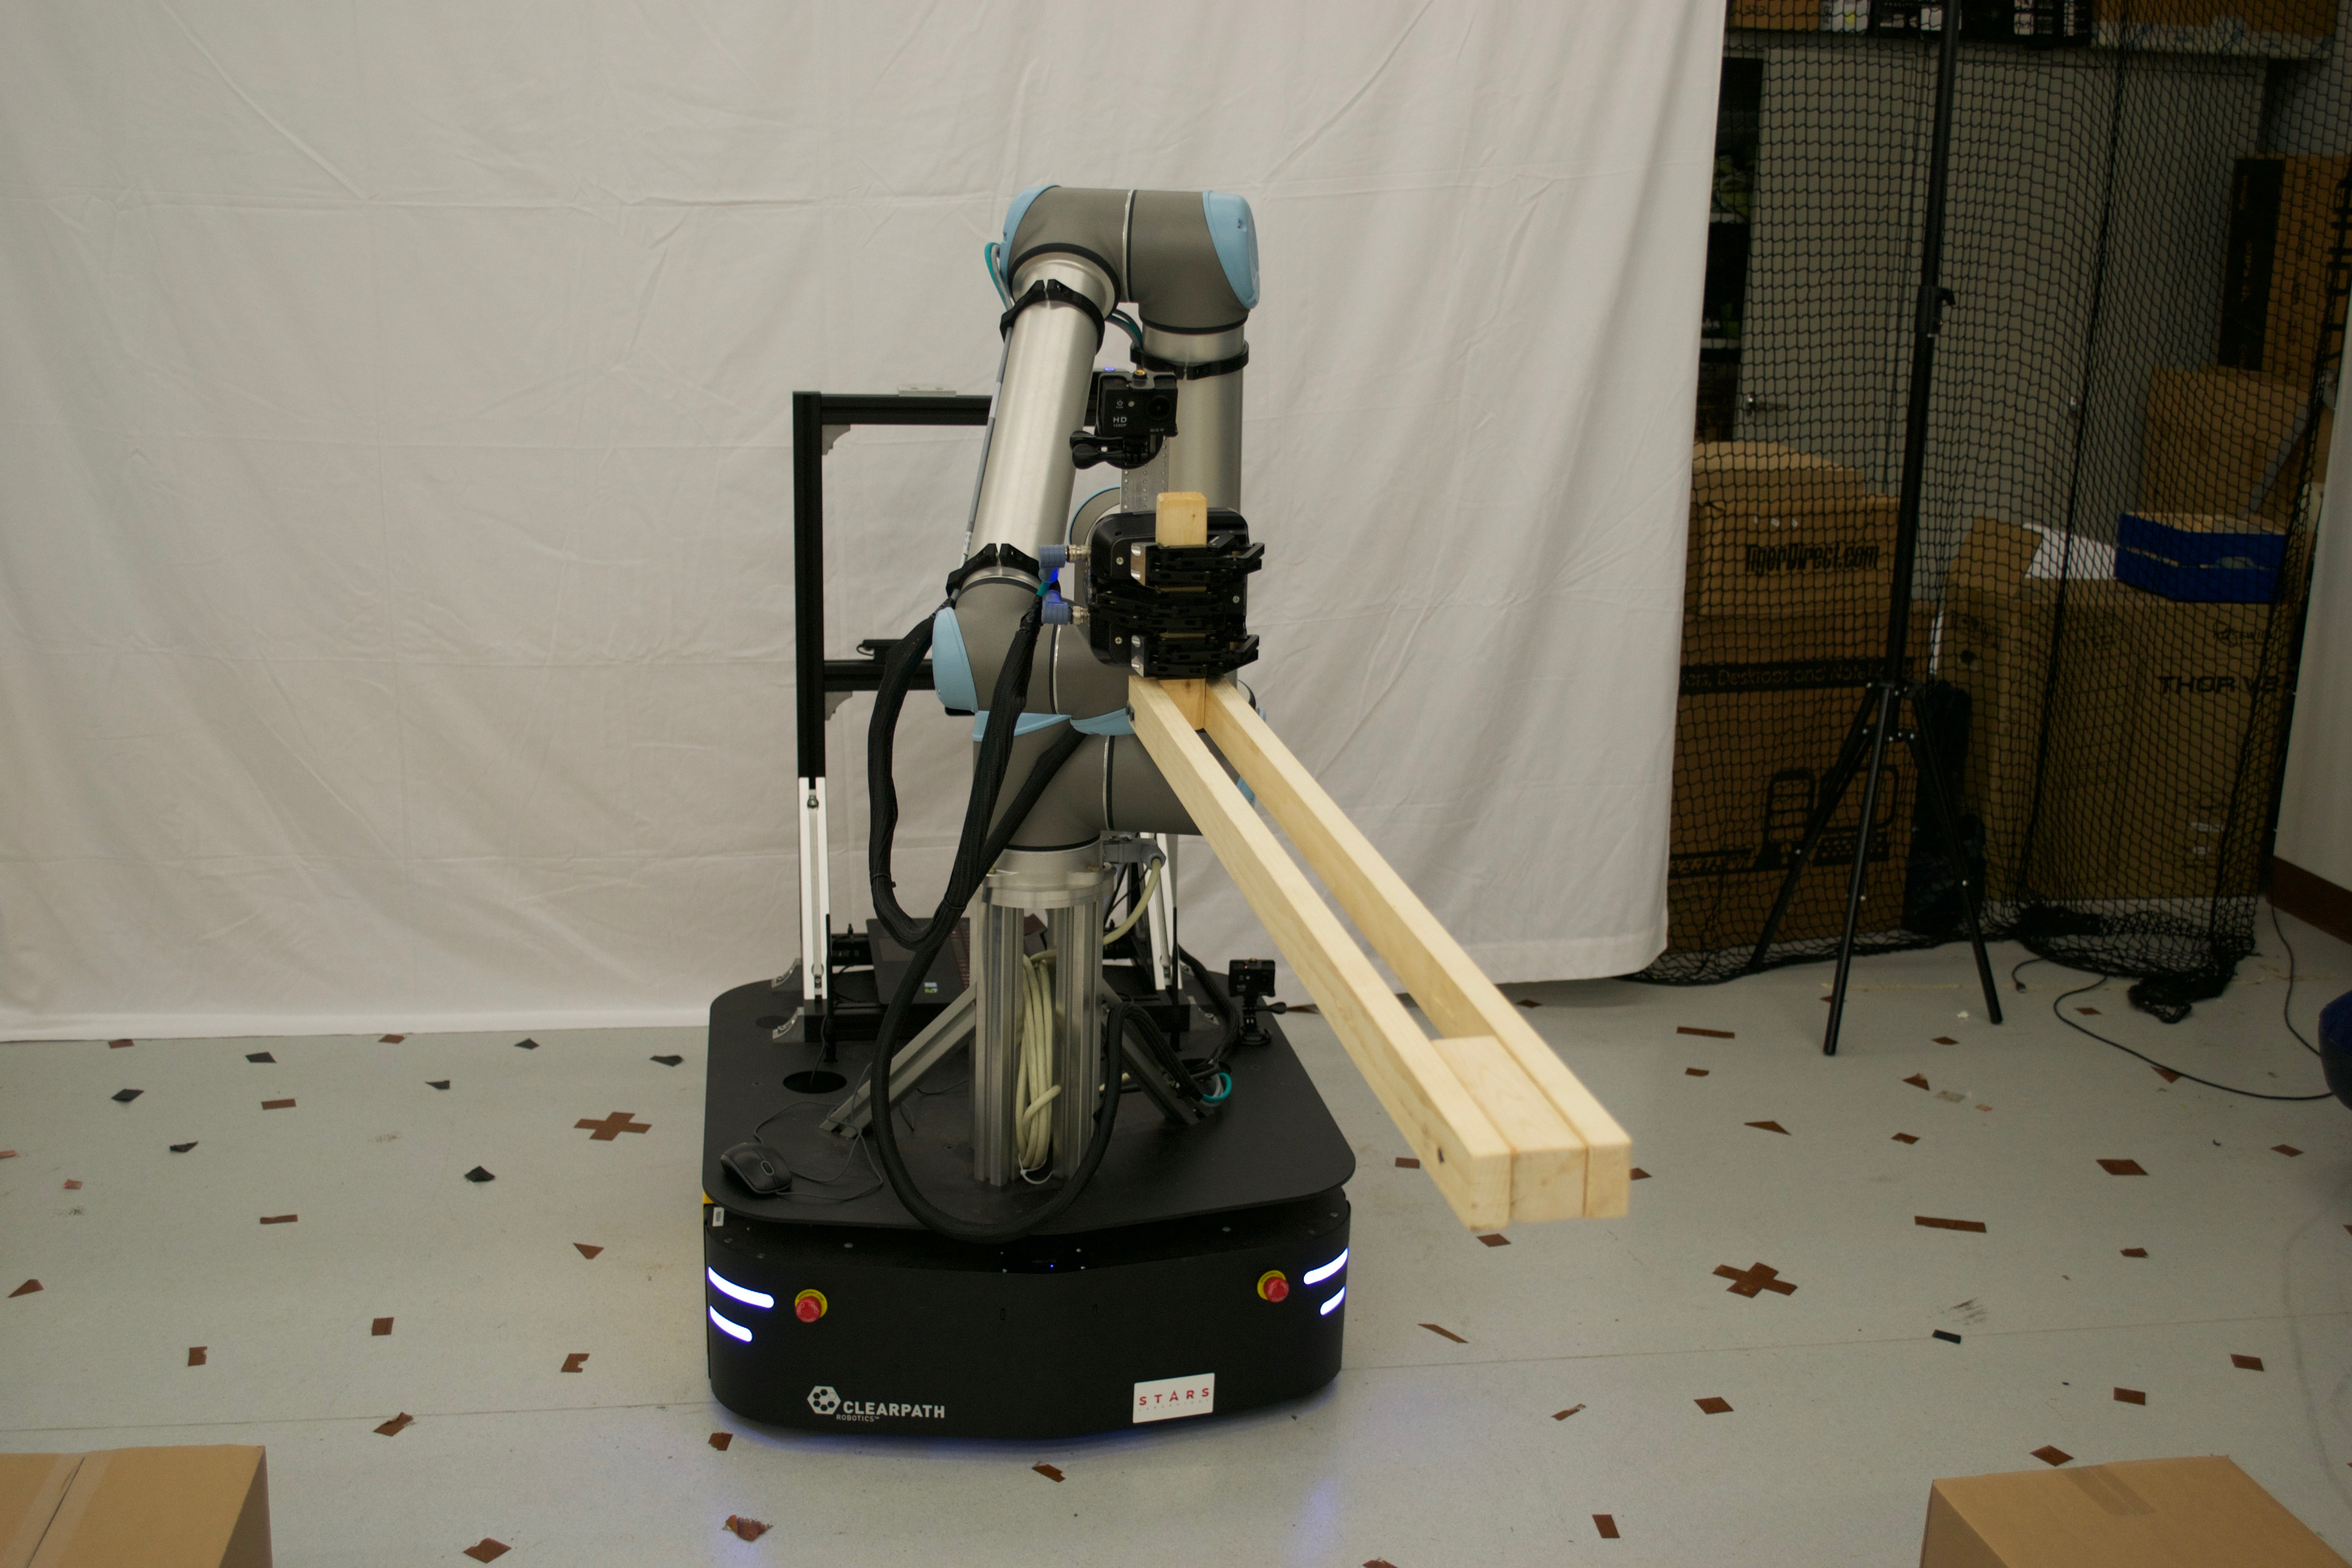
\includegraphics[width=0.75\textwidth]{images/test_setup.jpg}
   \caption{The Thing holding the jointly carried object used in the tests. It is a wooden structure three feet or \unit[91.44]{cm} in length and equipped with a handle to facilitate gripping.}
   \label{pics:test_setup}
\end{figure}

\section{Admittance Control Performance}
	\label{sec:adm_ctrl_performance}
As initial tests, we analyse the behaviour of the admittance controller in isolation. For this, we place the Thing in free space with no obstacles, i.e., in a region with zero gradient, so that the obstacle force $F_{obs} = 0$.

\begin{figure}
   \centering
   \includegraphics[width=\textwidth]{images/test18_x.jpg}
   \caption{Velocity response of both the base and the EE to force excitement in $x$.}
   \label{pics:test18_x}
\end{figure}

\begin{figure}
   \centering
   \includegraphics[width=\textwidth]{images/test18_y.jpg}
   \caption{Velocity response of both the base and the EE to force excitement in $y$.}
   \label{pics:test18_y}
\end{figure}

\begin{figure}
   \centering
   \includegraphics[width=\textwidth]{images/test18_theta.jpg}
   \caption{Velocity response  of both the base and the EE to torque excitement around $z$.}
   \label{pics:test18_theta}
\end{figure}

As seen in Chapter \ref{sec:params}, all six axes of our admittance controller are fully decoupled, therefore we can analyse the full behaviour of the admittance controller in the direction of an individual axis by applying force or torque on the object along the selected axis. We are most interested in the axes of the two mass spring damper system, i.e., the three axes that are within the DOF of the Ridgeback, so there is a response in both the Ridgeback and the EE. The three axes are linear $x$, linear $y$ and angular $z$ of the local base frame, where $x$ is pointing forward, $y$ to the right and $z$ upwards.

Figure \ref{pics:test18_x} depicts the velocity response of the system to a force excitement in $x$, Figure \ref{pics:test18_y} the response to a force excitement in $y$ and Figure \ref{pics:test18_theta} around $z$, i.e., the angular velocity $\theta$ given a torque input around $z$.

If we look at the response of the EE in both $x$, $y$ and $\theta$, we notice that it has a under-critically damped controller, which leads to a quick rise time and overshooting in the opposite direction, as soon as no more force is applied. This behaviour is desired, since we want to counteract sudden movement and jerky input by the human partner with the EE and only output smooth behaviour to the Ridgeback. If we have a look at the velocity response in $x$, $y$ and $\theta$ of the latter, we see a vastly slower rise time and no overshooting, i.e., a critically damped controller.

Furthermore, we notice that the linear velocity response of the EE peaks at \unitfrac[0.2]{m}{s} and the linear velocity response of the Ridgeback at \unitfrac[0.1]{m}{s}.

\section{Obstacle Avoidance and Admittance Control Performance}
Having the admittance controller tuned and working as desired, we can move on to testing the full algorithm where obstacle avoidance comes into play. We use cardboard boxes of dimension \unit[14 $\times$ 14 $\times$ 60]{inches} as obstacles, so that in case of a failure of the controller and an occurrence of a crash, the Thing does not get damaged.

Because we have no \unit[360]{\degree} \textsc{Lidar} coverage, but only a front-facing field of view, we can test the obstacle avoidance in forward and sideways motion of the Thing only. However, we've seen in Chapter \ref{sec:adm_ctrl_performance}, that the response to the admittance controller is independent of direction. Hence, we can assume that the full algorithm is scalable to a backward motion as well, if a back-facing \textsc{Lidar} were to be mounted.

\subsection{Frontal Obstacle}
The first obstacle avoidance test is the robot being pulled into an obstacle directly ahead of him. The scenario is depicted in Figure \ref{pics:test2_setup}. The velocity response of the system in the direction of pull, which is $x$, is plotted in Figure \ref{pics:test2}.

\begin{figure}
   \centering
   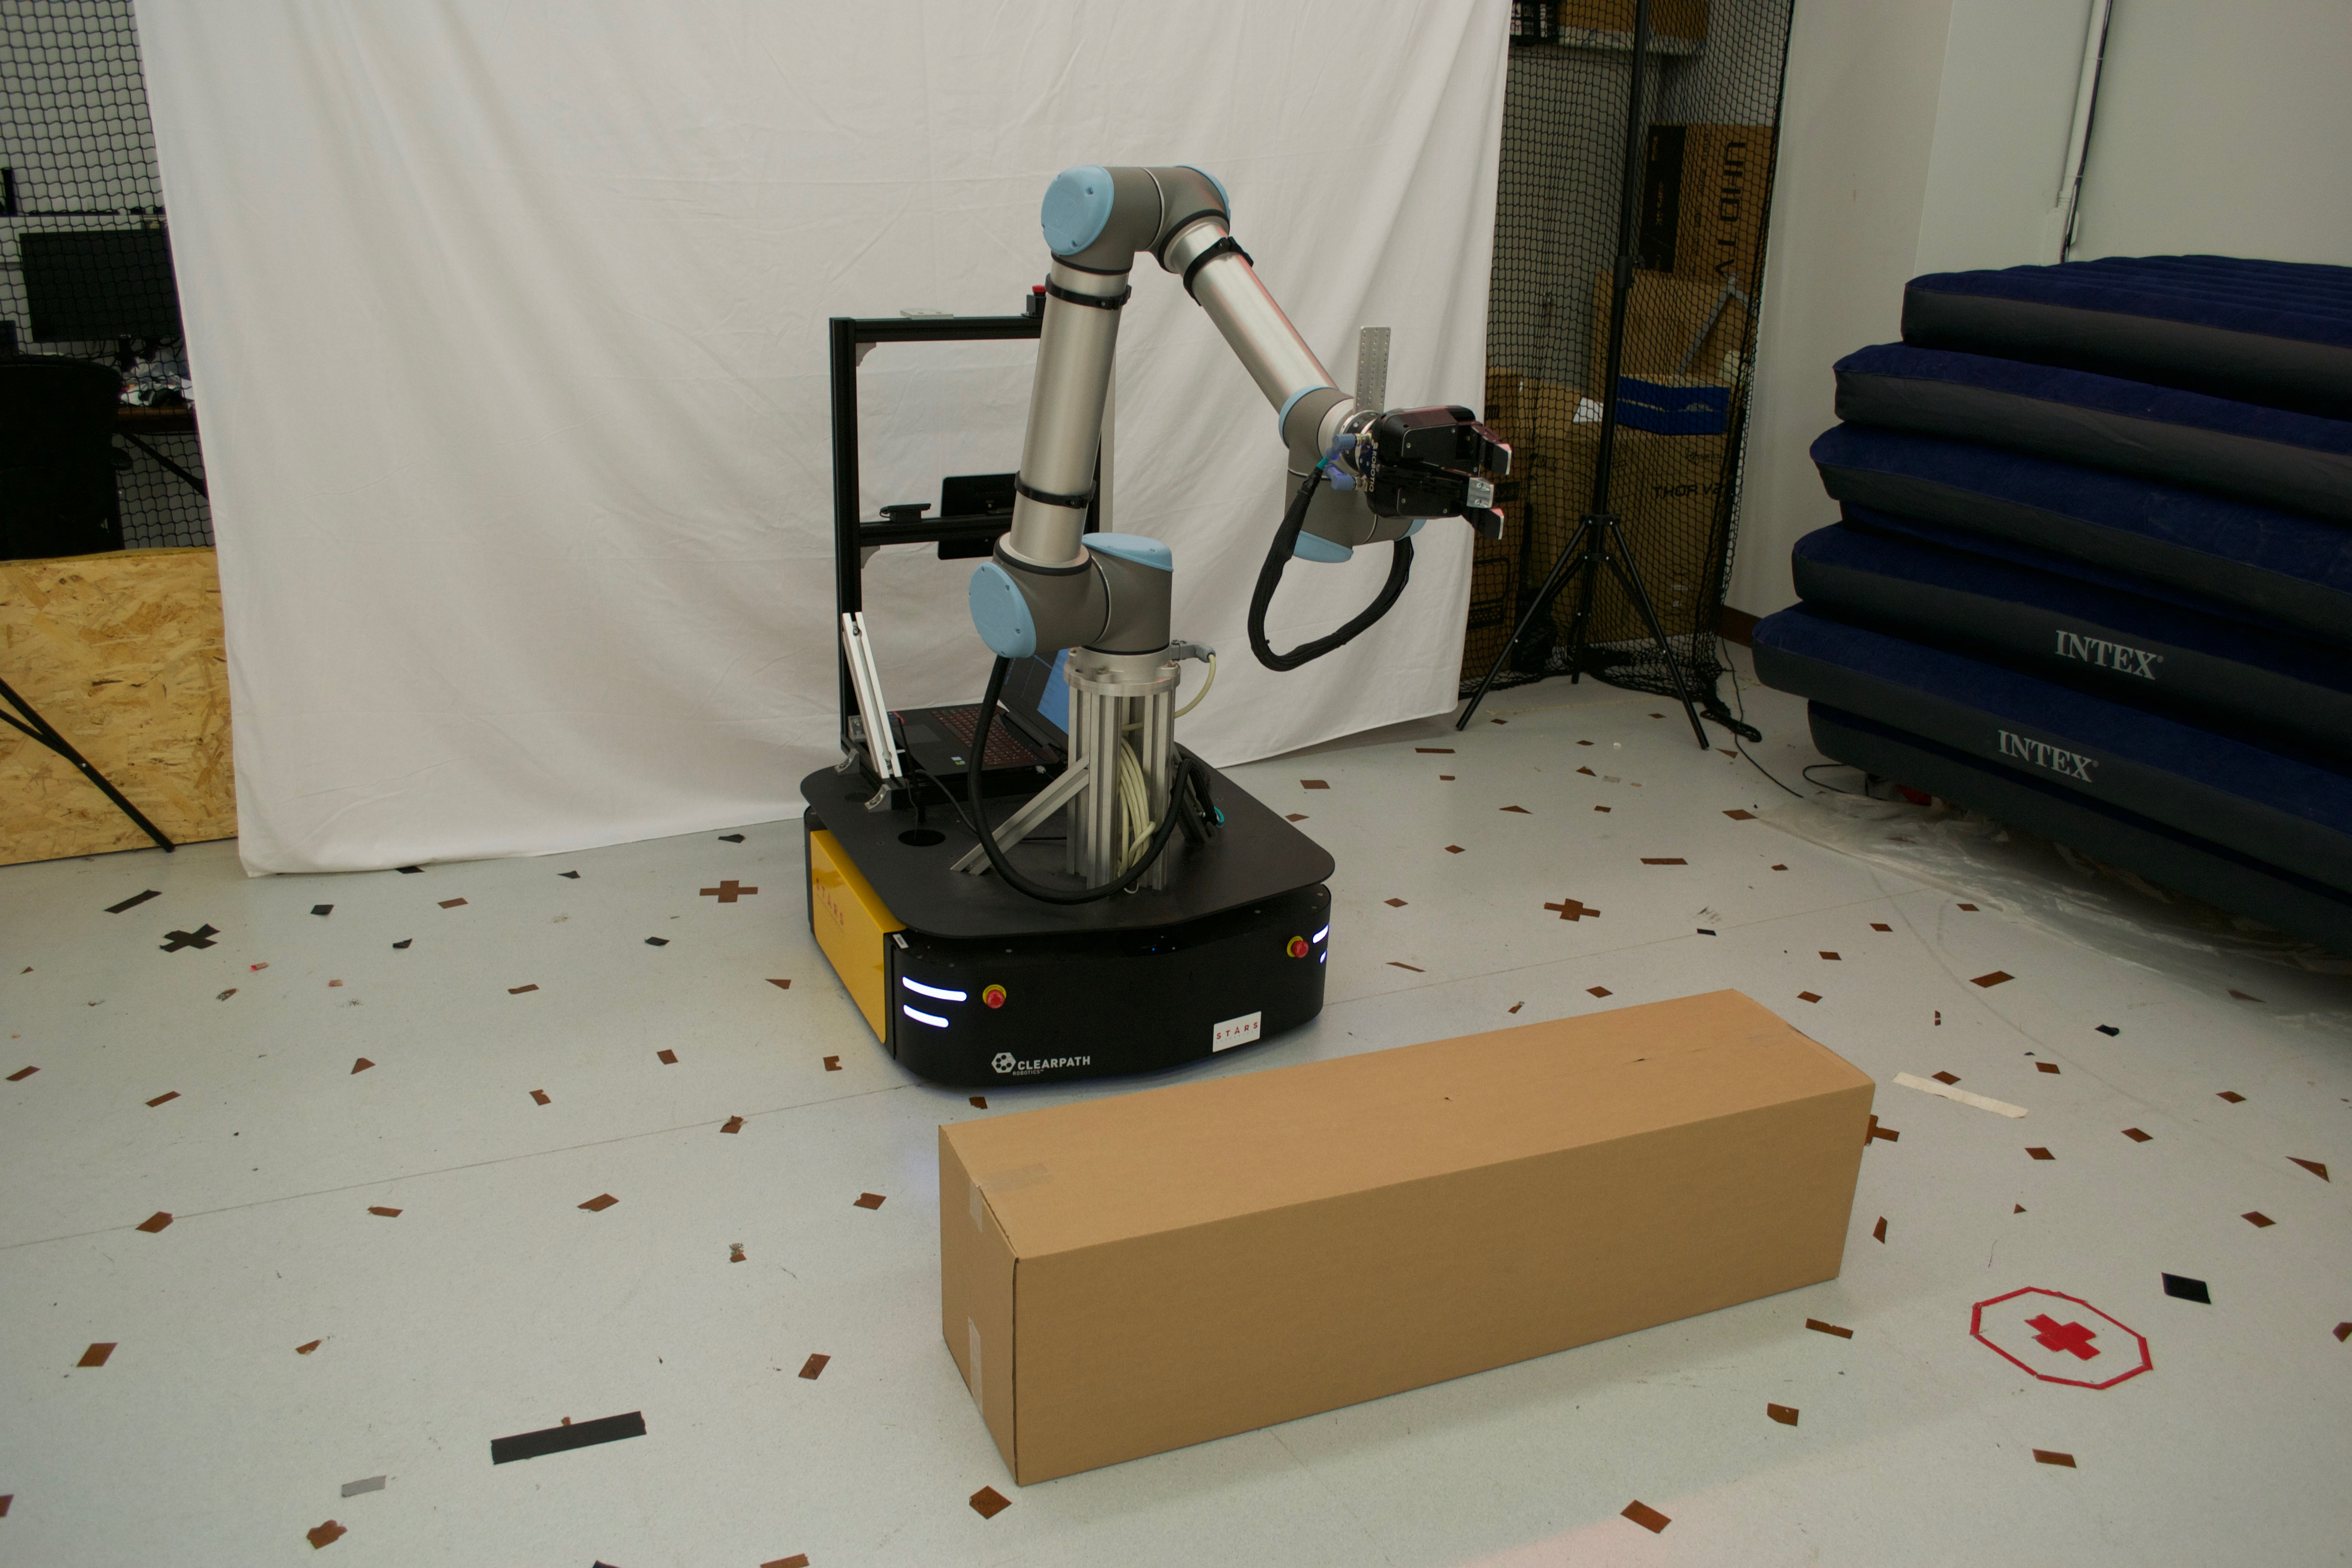
\includegraphics[width=0.75\textwidth]{images/test2_setup.jpg}
   \caption{Set-up of the frontal obstacle test scenario.}
   \label{pics:test2_setup}
\end{figure}

We see that the velocity responses of both EE and Ridgeback are constant, if a constant force is applied by the human partner and no obstacle is in range. However, as soon as we close in on the obstacle, the obstacle force pointing away from the obstacle rises and gradually diminishes the velocity responses to zero, although there is still a constant external force applied.

Figure \ref{pics:test2_costmap} depicts the cost map of the algorithm at the end of the experiment, i.e., at the robots closest position to the obstacle. We see the robot comes no closer than four grid cells to the obstacle, which equals a minimum obstacle clearance of \unit[12]{cm}. Together with the width of the Ridgeback of \unit[0.8]{m}, the lower bound on a narrow passage is thus slightly above\unit[1]{m}.

\begin{figure}
   \centering
   \includegraphics[width=\textwidth]{images/test2.jpg}
   \caption{Velocity response of both the base (\textsc{Black}) and the EE (\textsc{Black, dotted}) along the $x$ axis of the robot to external force $F_{ext}$ (\textsc{Red}) and obstacle force $F_{obs}$ (\textsc{Blue}) input while being pulled into a frontal obstacle.}
   \label{pics:test2}
\end{figure}

\begin{figure}
   \centering
   \includegraphics[width=\textwidth]{images/test2_costmap.jpg}
   \caption{Costmap at $t=34s$ of the frontal test. The range of the costmap is $[0,100]$, as explained in Chapter \ref{sec:costmap}, however we set the values of cells occupied by the robot base and by the obstacle ($c = 100$) to $c = 120$ for better readability (\textsc{Dark Red}).}
   \label{pics:test2_costmap}
\end{figure}

\subsection{Corner}

\begin{figure}
   \centering
   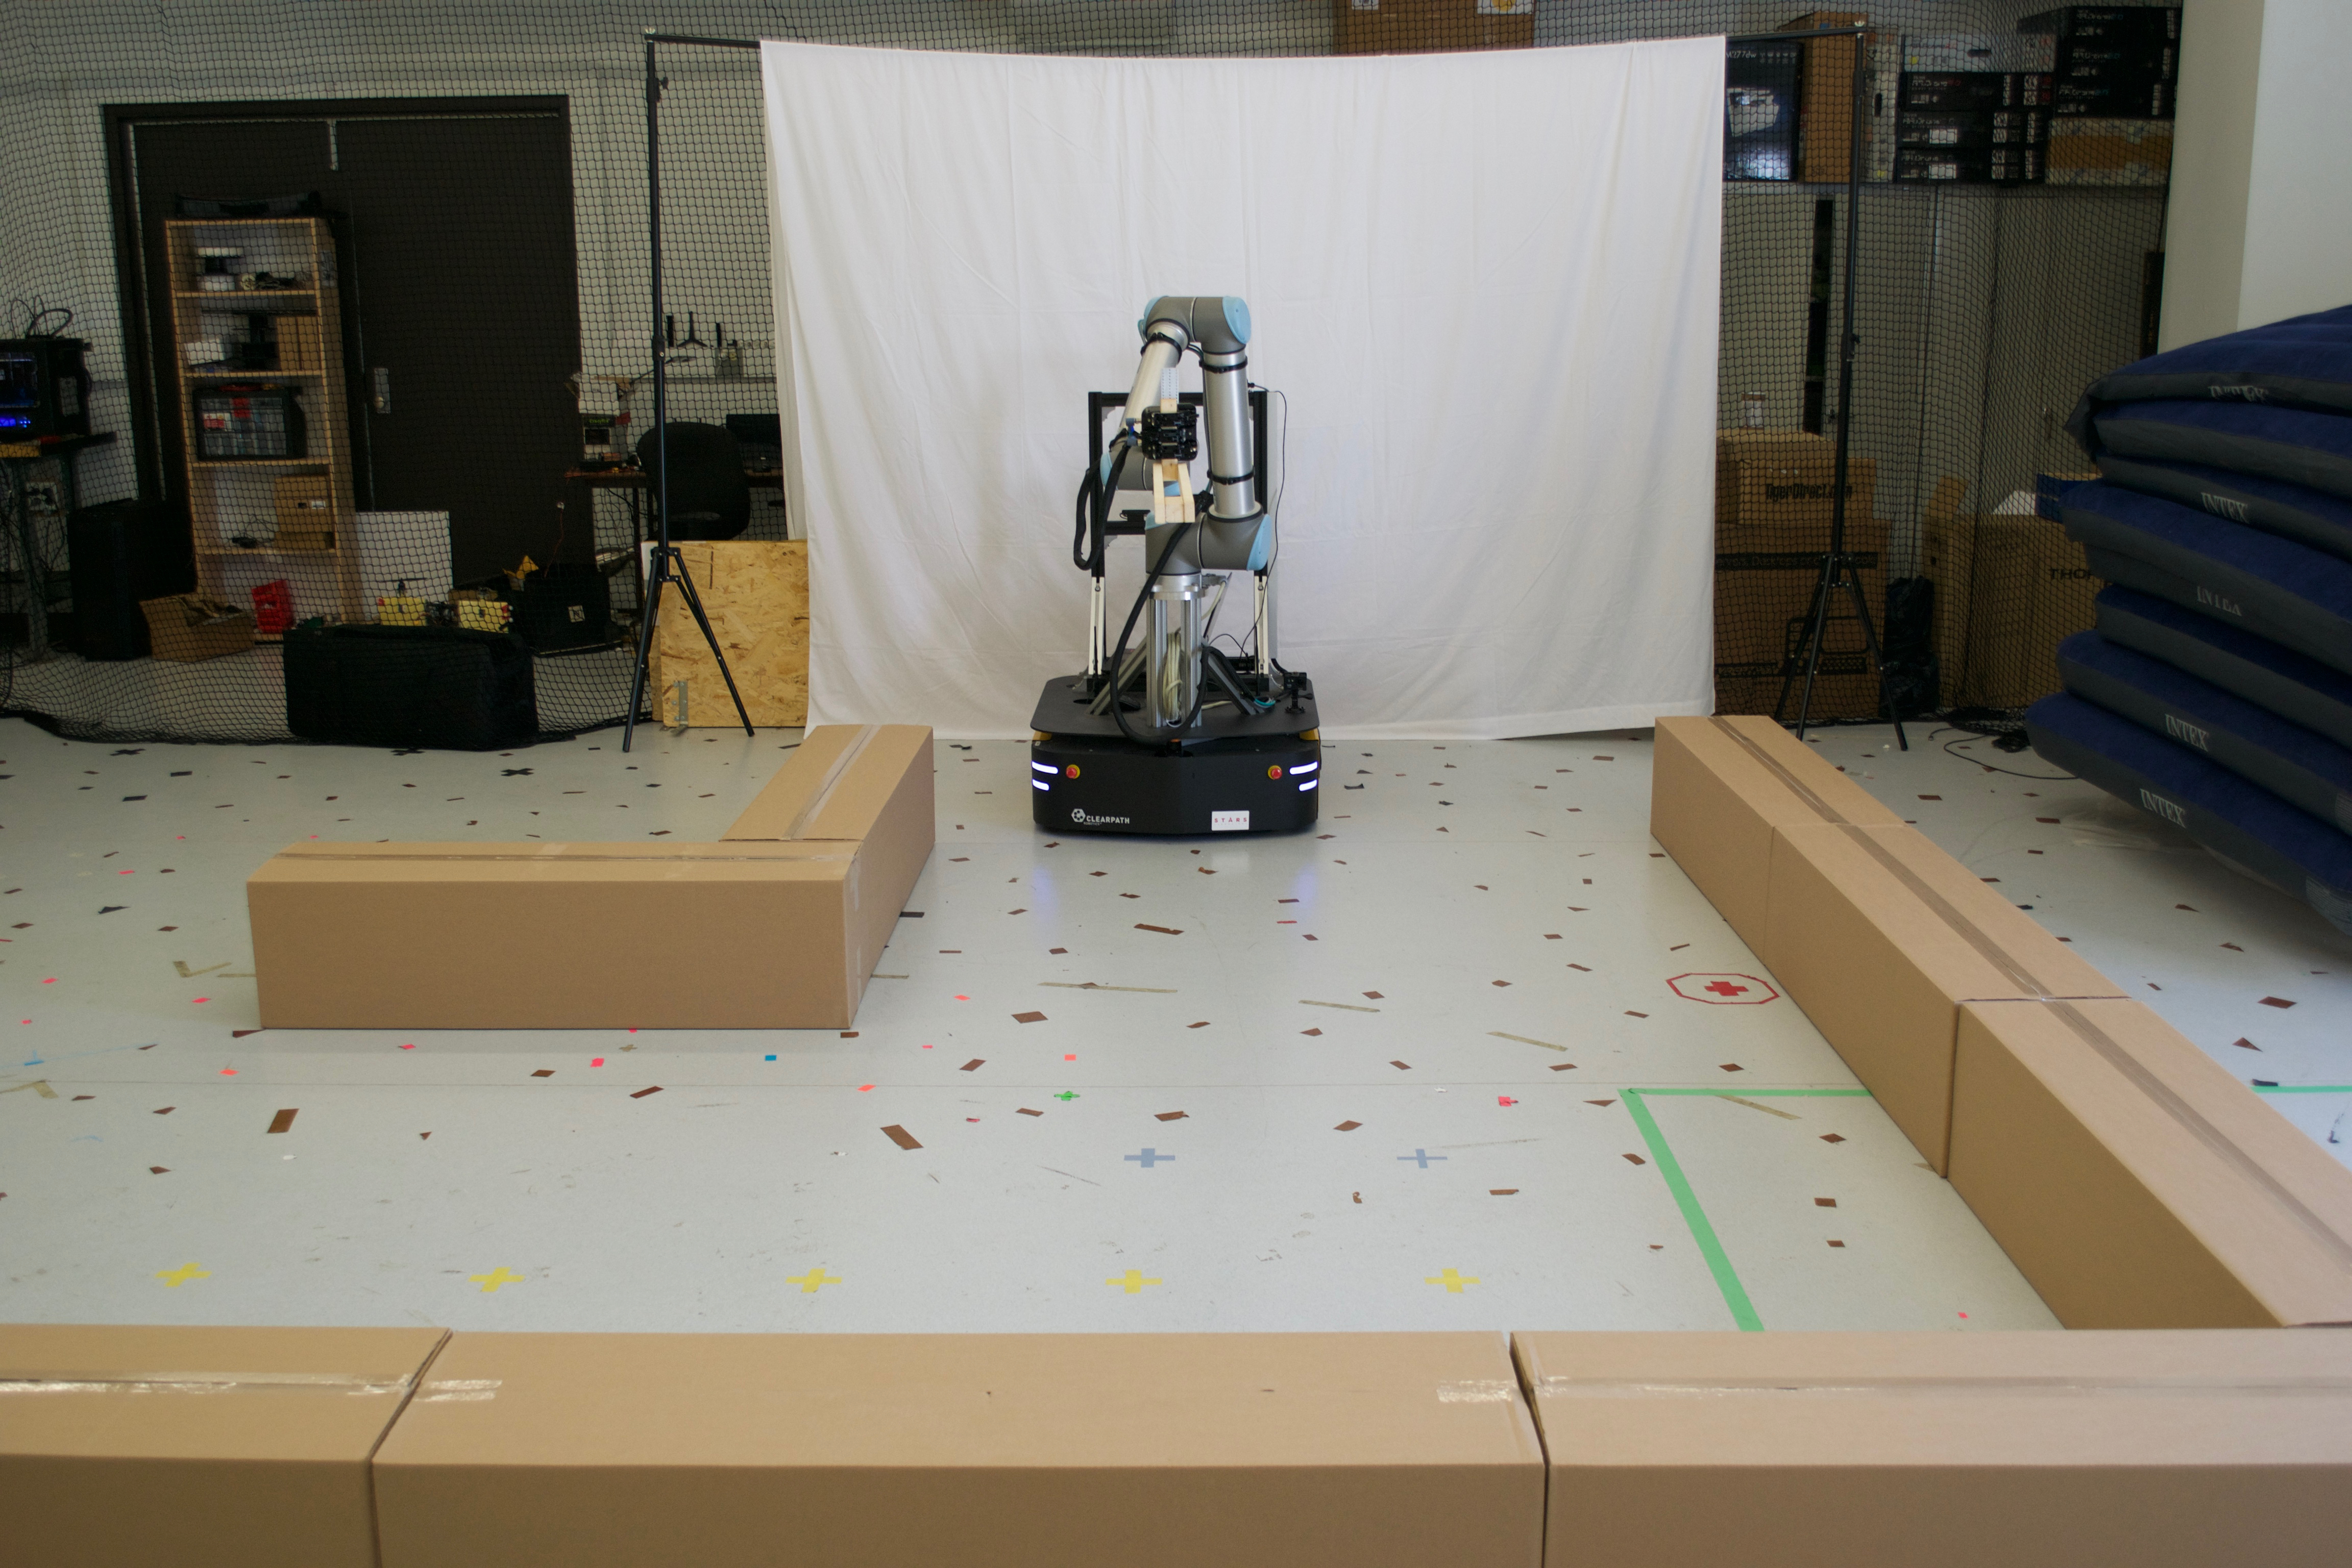
\includegraphics[width=0.75\textwidth]{images/test16_setup2.jpg}
   \caption{Set-up of the \unit{2}{m} wide corner scenario.}
   \label{pics:test16_setup}
\end{figure}

\begin{figure}
   \centering
   \includegraphics[width=\textwidth]{images/test16.jpg}
   \caption{Velocity response of both the base (\textsc{Black}) and the EE (\textsc{Black, dotted}) to external $F_{ext }$ (\textsc{Red}) and obstacle force $F_{obs}$ (\textsc{Blue}) input in \unit{2}{m} wide corner scenario. \textsc{Top} depicts the response along the $x$ axis and \textsc{Bottom} the response along the $y$ axis.}
   \label{pics:test16}
\end{figure}

In this experiment, we asses the performance of the algorithm in a corridor with a corner. The width of corridor is \unit{2}{m} and we jointly carry the object through it. The set-up at the beginning of the test is depicted in Figure \ref{pics:test16_setup}.

As we can see in Figure \ref{pics:test16}, there is a peak in the negative $y$ direction, which is caused by the robot drifting close to the outer wall as it is making the corner. This is due to the fact, that it is difficult for the human partner to apply torque in angular $z$, which makes the Thing rotate in place, without applying force in linear $y$, which makes the Thing move sideways. Hence, the trajectory of Ridgeback does not follow the center line of the hallway in a corner scenario, but rather utilizes the full width of the hallway.

\subsection{Cluttered Space}
As a final experiment, we test the behaviour in a cluttered environment, as seen in Figure \ref{pics:test16_setup}. It consists of four boxes in a perpendicular arrangement with the last two boxes forming a passage of \unit[120]{cm} width.

In Figure \ref{pics:test15}, we notice the first box to which the Thing gets close as a repulsive force at $t = 26s$, which leads to a deviation in negative $y$ of the base from the path defined by $F_{ext}$. And when passing through the narrow passage at $t = 95s$, we see a slight oscillation in $F_{obs}$ in $y$, because the base is coming close to an obstacle on either side and needs to settle down on the optimal gradient centreline in between.

\newpage

\begin{figure}
   \centering
   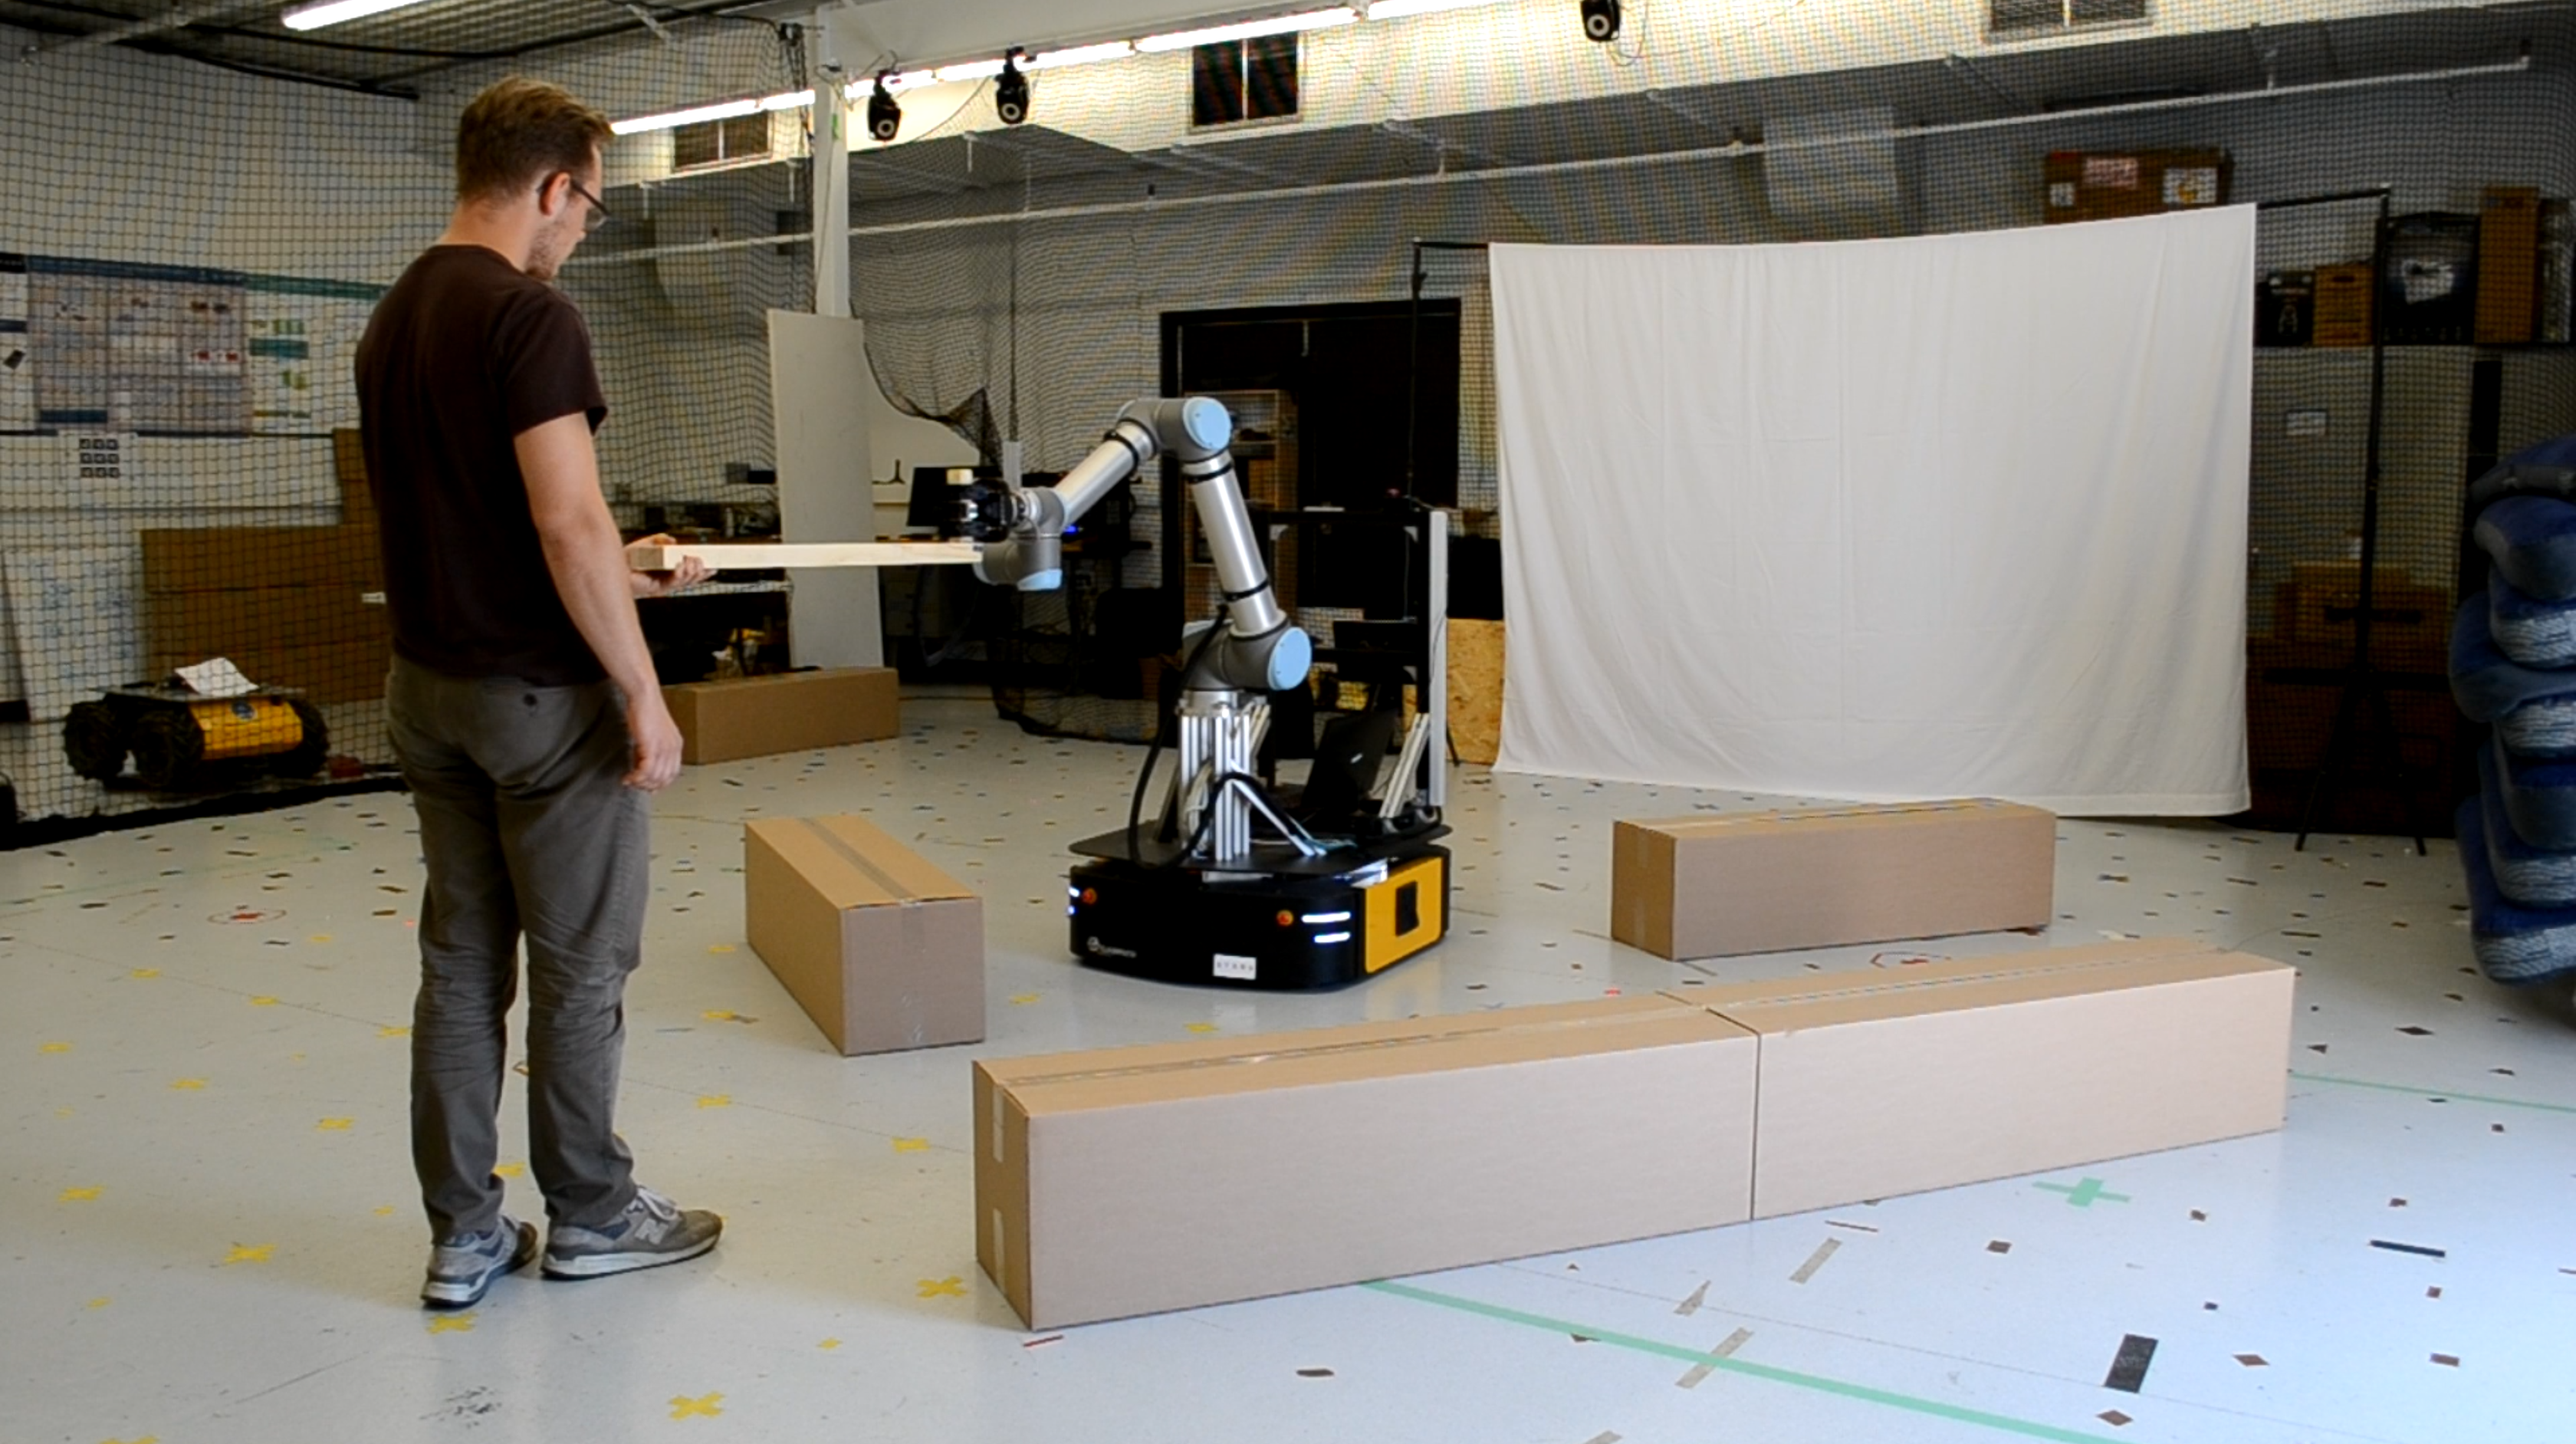
\includegraphics[width=0.75\textwidth]{images/test15_setup.png}
   \caption{Execution of a test in the cluttered environment scenario.}
   \label{pics:test15_setup}
\end{figure}

\begin{figure}
   \centering
   \includegraphics[width=\textwidth]{images/test15_response.jpg}
   \caption{Velocity response of both the base (\textsc{Black}) and the EE (\textsc{Black, dotted}) to external $F_{ext }$ (\textsc{Red}) and obstacle force $F_{obs}$ (\textsc{Blue}) input in \unit{2}{m} cluttered environment scenario. \textsc{Top} depicts the response along the $x$ axis and \textsc{Bottom} the response along the $y$ axis.}
   \label{pics:test15}
\end{figure}

\chapter{Discussion}
In this work, we successfully demonstrate a load-sharing algorithm that utilizes an admittance controller and an obstacle avoidance algorithm for a mobile manipulator in collaboration with a human partner. Through usage of the potential field method for obstacle avoidance, we achieve an unified controller that incorporates both the input of the human as an attractive external force and the input of the obstacle avoidance as a repulsive force into the two mass spring damper system which is the core of the algorithm. The robot has no need for a prior map of the environment and can evade static and dynamic obstacles alike.

As the experimental results show, the implementation on a mobile manipulator, consisting of a Ridgeback base and a UR10 manipulator, proves the feasibility of the control architecture. We run the system at \unit[125]{Hz} and achieve a clearance of \unit[12]{cm} for the base around any obstacles, while complying with the input of the human partner. The robot demonstrates a pro-active behaviour, both in scenarios with one obstacle and environments that are cluttered. The robot guides the human partner away from detected obstacles and guarantees no collision, independent of the human input. Furthermore, we achieve a smooth and intuitive motion cooperation, which can be greatly adapted and personalized through tuning of the damping and the spring parameters.

Simultaneously, the data from the experiments also shows the limitations of the system. For one, because there is only a front facing \textsc{Lidar}, the Ridgeback can only evade obstacles in forward and sideways motion, which can easily be overcome with additional hardware. A more fundamental limitation of the obstacle avoidance is the fact that the potential field method does not propose a direction of motion, if the external force $F_{ext}$ of the human is parallel to the local gradient. In that case, the resulting velocity is only increased or decreased, but does not change direction. Hence, in a scenario where an obstacle is encountered with a face perpendicular to the direction of the external force, the human partner has to give additional force input to overcome said obstacle. Here, a path planning or intent recognition based on the position of the human partner, as seen by the \textsc{Lidar}, could be an improvement to the system.

Also, the width of the most narrow passage through which the robot can travel could be decreased by alteration of the potential field cost function. This is because the width is currently limited by a static oscillation perpendicular to the direction of travel, that the robot exhibits when passing a narrow corridor. The oscillation is caused by the superposition of the cost of both obstacles, which leads to a discontinuous total cost. Smoothing of the total cost can be considered to minimize this oscillation.

Lastly, the maximal achieved velocity is no more than \unitfrac[0.3]{m}{s} for the robot base, which is to be improved before this system can be applied in a real-world scenario, e.g. a factory.

In conclusion, this work does not derive a novel algorithm, but rather combines and implements existing concepts on a real platform. It shows the advantages of human-robot cooperation in a load-sharing scenario, since the robot not only takes physical load off the human but also cognitive load by guiding the human partner away from obstacles. The next step would be to reach full human-robot cooperation, where for example the robot makes active decisions in terms of where to place the jointly carried object or guides the human towards a goal.